
\documentclass{beamer} 


\mode<presentation>
{
  \usetheme[hideothersubsections]{Berkeley}
  % or ...

  \setbeamercovered{transparent}
  % or whatever (possibly just delete it)
}

\usepackage{tikz}
\usepackage{graphicx}
\usepackage[english]{babel}
\usepackage{tikz}
\usetikzlibrary{decorations.pathreplacing,angles,quotes}
\usetikzlibrary{shapes, shadows, arrows, positioning,fit}
\usepackage{multirow, booktabs, adjustbox}
\usepackage{relsize, lscape}
\usepackage[utf8]{inputenc}
\usepackage{adjustbox}
\usepackage{verbatim}
\usepackage{listings, amsmath}
\usepackage{natbib}
\usepackage{tcolorbox}
\usepackage{transparent}


\usepackage{relsize, lscape}
\usepackage{multirow, booktabs, adjustbox}
\usepackage{lipsum} % Used for inserting dummy 'Lorem ipsum' text into the template
\usepackage{array}
\usepackage{graphicx}
\usepackage{hyperref}


% or whatever

\usepackage{times}
\usepackage[T1]{fontenc}
% Or whatever. Note that the encoding and the font should match. If T1
% does not look nice, try deleting the line with the fontenc.


\addtobeamertemplate{navigation symbols}{}{%
    \usebeamerfont{footline}%
    \usebeamercolor[fg]{footline}%
    \hspace{1em}%
    \insertframenumber/\inserttotalframenumber
}

\newcommand{\nit}[1]{\textrm{\textit{{\color{red}[#1]}}}}
\newcommand{\highlight}[1]{\colorbox{yellow}{$\displaystyle #1$}}
\newcommand{\highlightw}[1]{\colorbox{white}{$\displaystyle #1$}}
\newcommand{\tabitem}{~~\llap{\textbullet}~~}


\def\gray{\color{lightgray}}
\def\red{\color{red}}
\def\white{\color{white}}
\def\brown{\color{brown}}
\def\black{\color{black}}
\def\blue{\color{blue}}



\renewcommand{\topfraction}{0.9}
\newsavebox{\codebox}
\lstset{
basicstyle=\scriptsize\tt,
}

\newcolumntype{P}[1]{>{\raggedright\arraybackslash}p{#1}}

\newcommand{\backupbegin}{
   \newcounter{finalframe}
   \setcounter{finalframe}{\value{framenumber}}
}
\newcommand{\backupend}{
   \setcounter{framenumber}{\value{finalframe}}
}

\newcommand\Wider[2][3em]{%
\makebox[\linewidth][c]{%
  \begin{minipage}{\dimexpr\textwidth+#1\relax}
  \raggedright#2
  \end{minipage}%
  }%
}
%control cross slide button format
\setbeamertemplate{button}{\tikz
  \node[
  inner xsep=2pt,
  draw=structure!50,
  fill=structure!50,
  rounded corners=2pt]  {\Large\insertbuttontext};}


\title[OPA - Minimum Wage ] % (optional, use only with long paper titles)
{Open Policy Analysis: A Case Study of the Minimum Wage Policy Estimate}

\subtitle
{}

\author[] % (optional, use only with lots of authors)
{Fernando~Hoces de la Guardia\inst{1}}
% - Give the names in the same order as the appear in the paper.
% - Use the \inst{?} command only if the authors have different
%   affiliation.

\institute[Universities of Somewhere and Elsewhere] % (optional, but mostly needed)
{
  \inst{1}%
  UC Berkeley:\\
  Berkeley Initiative for Transparency in the Social Sciences\\
}
% - Use the \inst command only if there are several affiliations.
% - Keep it simple, no one is interested in your street address.

\date[] % (optional, should be abbreviation of conference name)
{Congressional Budget Office, March 2018\\
{\small Slides at} \url{http://www.github.com/fhoces/CBO2018}}
% - Either use conference name or its abbreviation.
% - Not really informative to the audience, more for people (including
%   yourself) who are reading the slides online

\subject{Research Transparency}
% This is only inserted into the PDF information catalog. Can be left
% out. 

\pgfdeclareimage[height=2cm]{university-logo}{../Images/BITSSlogo.png}
\logo{\pgfuseimage{university-logo}}

% If you have a file called "university-logo-filename.xxx", where xxx
% is a graphic format that can be processed by latex or pdflatex,
% resp., then you can add a logo as follows:

% \pgfdeclareimage[height=0.5cm]{university-logo}{university-logo-filename}
% \logo{\pgfuseimage{university-logo}}



% Delete this, if you do not want the table of contents to pop up at
% the beginning of each subsection:
%\AtBeginSubsection[]
%{
%  \begin{frame}<beamer>{Outline}
%    \tableofcontents[currentsection,currentsubsection]
%  \end{frame}
%}


% If you wish to uncover everything in a step-wise fashion, uncomment
% the following command: 

\beamerdefaultoverlayspecification{<.->}


\begin{document}

\begin{frame}
  \titlepage
\end{frame}

\begin{frame}{Outline}
  \tableofcontents
  % You might wish to add the option [pausesections]
\end{frame}
 
\section{Motivation}

\begin{frame}{Motivation}
\begin{itemize}
\item Manski
\item Report Wars
\item Hoces de la Guardia, Grant \& Miguel
\end{itemize}
\end{frame}
 
\begin{frame}{Ideal Connection Between Evidence and Policy}



\tikzstyle{agent} = [diamond, draw, node distance= 7em, minimum height=5em, minimum width=5em]
\tikzstyle{line} = [draw, -stealth]

\tikzstyle{line_enph} = [draw, red, ultra thick]
\tikzstyle{inp} = [draw, circle, text centered, minimum height=2em, text width=2em, node distance= 10em]
\tikzstyle{outp} = [draw, circle, text centered, minimum height=2em, text width=2em, node distance= 10em]
\tikzstyle{block1} = [draw, circle,  text width=5em, text centered, minimum height=7em, node distance= 5em]
\tikzstyle{block2} = [draw, circle,  text width=7em, text centered, minimum height=2em, node distance= 5em]
\tikzstyle{block3} = [draw, rounded rectangle,  text width=5em, text centered, minimum height=2em, node distance= 5em]


\begin{figure}[h!]\centering
\vspace{-2.0em}
\begin{tikzpicture}[thick,scale=0.55, every node/.style={scale=0.55}]

%% The oddly shaped truth
\node[regular polygon, regular polygon sides=3,
              draw, fill=white,
              inner sep=.1em,
              shape border rotate=70](tru){Truth};


%%%%%Researcher 1 and Inputs: depends on R_1%%%%%%%
\node [block1, right = 2em of tru](R_1){Research\linebreak $(R)$};
\node [block1,inner sep=0em, right = 2em of R_1](PA_1){Policy \linebreak Analysis: ($PA$) \linebreak  Gains  \& \linebreak losses};
\node [block1, above right = 0em and 8em of R_1](PM_1){Policy\linebreak Maker 1};
\node [block1, below right = 0em and 8em of R_1](PM_2){Policy\linebreak Maker 2};

\node [block3, right = 2em of PM_1](PC_1){Support};
\node [block3, right = 2em of PM_2](PC_2){Oppose};


%%%%% Draw edges col 2%%%%%%%%%%%%%%%%%
%Research  to PA
\draw [line](tru) -- (R_1);
\draw [line](R_1) -- (PA_1);
%PA to PM
\draw [line](PA_1) -- (PM_1);
\draw [line](PA_1) -- (PM_2);
%PM to PC
\draw [line](PM_1) -- (PC_1);
\draw [line](PM_2) -- (PC_2);

%%%%%%%%%%%%%%%%%%%%%%%%%%%%%%%%%%%%%%



\draw[decoration={brace}, decorate] (7,3.4) -- node[above=6pt](lab4){{\Large Observed by citizens} }(16,3.4);




\end{tikzpicture}
\vspace{-.8em}
\end{figure}
\end{frame}






\begin{frame}[shrink=30]{Current Connection Between Evidence and Policy}



\tikzstyle{agent} = [diamond, draw, node distance= 7em, minimum height=5em, minimum width=5em]
\tikzstyle{line} = [draw, -stealth]

\tikzstyle{line_d} = [draw, dashed, -stealth]
\tikzstyle{inp} = [draw, circle, text centered, minimum height=2em, text width=2em, node distance= 10em]
\tikzstyle{outp} = [draw, circle, text centered, minimum height=2em, text width=2em, node distance= 10em]
\tikzstyle{block1} = [draw, circle,  text width=3em, text centered, minimum height=2em, node distance= 5em]
\tikzstyle{block2} = [draw, circle,  text width=4em, text centered, minimum height=2em, node distance= 5em]
\tikzstyle{block3} = [draw, rounded rectangle,  text width=5em, text centered, minimum height=2em, node distance= 5em]

\begin{figure}[h!]
\centering
\hspace*{0.2\linewidth}
\begin{tikzpicture}[thick,scale=0.2, every node/.style={scale=0.8}]

%% The oddly shaped truth
\node[regular polygon, regular polygon sides=3,
              draw, fill=white,
              inner sep=.1em,
              shape border rotate=70](tru){Truth};


%%%%%Researcher 1 and Inputs: depends on R_1%%%%%%%
\node [block1, right = 5em of tru](R_2){$R_2$};
\node [block1, above = 8em of R_2](R_1){$R_1$} node [left = -0.1em of R_1, text width = 5em]{Large Treatment Effect};
\node [block1, below = 8em of R_2](R_3){$R_3$} node [left = -0.1em of R_3, text width = 5em]{Small Treatment Effect};

\draw[decoration={brace,mirror}, decorate] (13,-33) -- node[below=6pt, text width = 4.8em](lab1){Researchers Degrees of 
Freedom}(18,-33);

\draw[decoration={brace,mirror}, decorate] (29,-33) -- node[below=6pt, text width = 5em](lab2){Policy Analyst Degrees of 
Freedom}(34,-33);

\draw[decoration={brace}, decorate] (31,33) -- node[below=2pt]{Observed by citizens}(70,33);

%\node [agent](Researcher_1){$R_1$} node [left = 0.6em of Researcher_1, text width = 8em]{Large Treatment Effect};

\node [block1, right = 5em of R_1](PA_12){$PA_{1,2}$};
\node [block1, above = .5em of PA_12](PA_11){$PA_{1,1}$} node [right = -0.1em of PA_11, text width = 5em]{Large gains only};
\node [block1, below = .5em of PA_12](PA_13){$PA_{1,3}$};

\node [block1, right = 5em of R_2](PA_22){$PA_{22,}$};
\node [block1, above = .5em of PA_22](PA_21){$PA_{2,1}$};
\node [block1, below = .5em of PA_22](PA_23){$PA_{2,3}$};

\node [block1, right = 5em of R_3](PA_32){$PA_{3,2}$};
\node [block1, above = .5em of PA_32](PA_31){$PA_{3,1}$};
\node [block1, below = .5em of PA_32](PA_33){$PA_{3,3}$} node [right = -0.1em of PA_33, text width = 5em]{Large losses only};


\node [block2, above right = 3em and 15em of R_2](PM_1){Policy\linebreak Maker 1};
\node [block2, below right = 3em and 15em of R_2](PM_2){Policy\linebreak Maker 2};

\node [block3, right = 3em of PM_1](PC_1){Support};
\node [block3, right = 3em of PM_2](PC_2){Oppose};


%%%%% Draw edges col 2%%%%%%%%%%%%%%%%%
%Truth to research
\draw [line](tru) -- (R_1);
\draw [line_d](tru) -- (R_2);
\draw [line_d](tru) -- (R_3);


%Research  to PA
\draw [line_d](R_1) -- (PA_13);
\draw [line_d](R_1) -- (PA_11);
\draw [line](R_1) -- (PA_12);

\draw [line_d](R_2) -- (PA_23);
\draw [line_d](R_2) -- (PA_21);
\draw [line_d](R_2) -- (PA_22);

\draw [line_d](R_3) -- (PA_33);
\draw [line_d](R_3) -- (PA_31);
\draw [line_d](R_3) -- (PA_32);



%PA to PM
\draw [line](PA_11) -- (PM_1);
\draw [line](PA_33) -- (PM_2);
%PM to PC
\draw [line](PM_1) -- (PC_1);
\draw [line](PM_2) -- (PC_2);

%%%%%%%%%%%%%%%%%%%%%%%%%%%%%%%%%%%%%%




\end{tikzpicture}
\end{figure}
%\end{comment}
\end{frame}



  
 
 \section{Approach}
\begin{frame}{Approach}
\begin{itemize}
\item Identify a case study
\item Define guidelines
\item Demonstrate how to achieve highest standards of OPA
\item Use sensitivity analysis to explore biggest policy unknowns 
\begin{itemize}
\item  Surprisingly academic debate around one specific parameter seems less relevant from policy perspective
\end{itemize}
\end{itemize}
\end{frame} 

\section[Case Study]{Description of Case Study}

\begin{frame}[label =  desc_cs]{Description of Case study}
% 4mins
\begin{center}
``The Effects of a Minimum-Wage Increase on Employment and Family Income'' 
Congressional Budget Office (2014)
\end{center}

\textbf{Description:} CBO estimated the effects of a raise in the federal minimum wage from \$7.25/hr to \$10.10/hr. 


\textbf{Main policy estimates:}
\begin{itemize}
\item ~500,000 jobs would be lost.
\item 16.5 million workers would receive a salary increase. 
\item Distributional effects: below poverty line (PL) +\$5billion; between one and three PL +\$12billion; between three and six PL +\$2billion; above six PL -\$17billion
\end{itemize}

\textbf{Key research estimate:} Elasticity of labor demand for teenagers in the labor force. 
\end{frame}



\begin{frame}[label = reas_cs]{Reasons for Selecting the Case Study}
\vspace*{1em}
\begin{itemize}
\item \textit{Scalable}: CBO's reputation: among the most transparent and rigorous policy analysis offices. Lessons from TR that apply to CBO should apply also to most agencies.  Additionally the policy issue is widely known which facilitates parallels. 
\item \textit{Recurrent}: This policy analysis will be conducted again in the future. The case study can be directly used in future calculations. 
\end{itemize}

\end{frame}

\begin{frame}{Reasons for Selecting the Case Study}

\begin{itemize}
\item \textit{Feasible}: available data, good description of the analysis, and only one policy lever to analyze. 
\item \textit{Relevant}: 
\end{itemize}

\begin{figure}[h!]
\centering
\vspace*{-1em}
\hspace*{-1.7em}
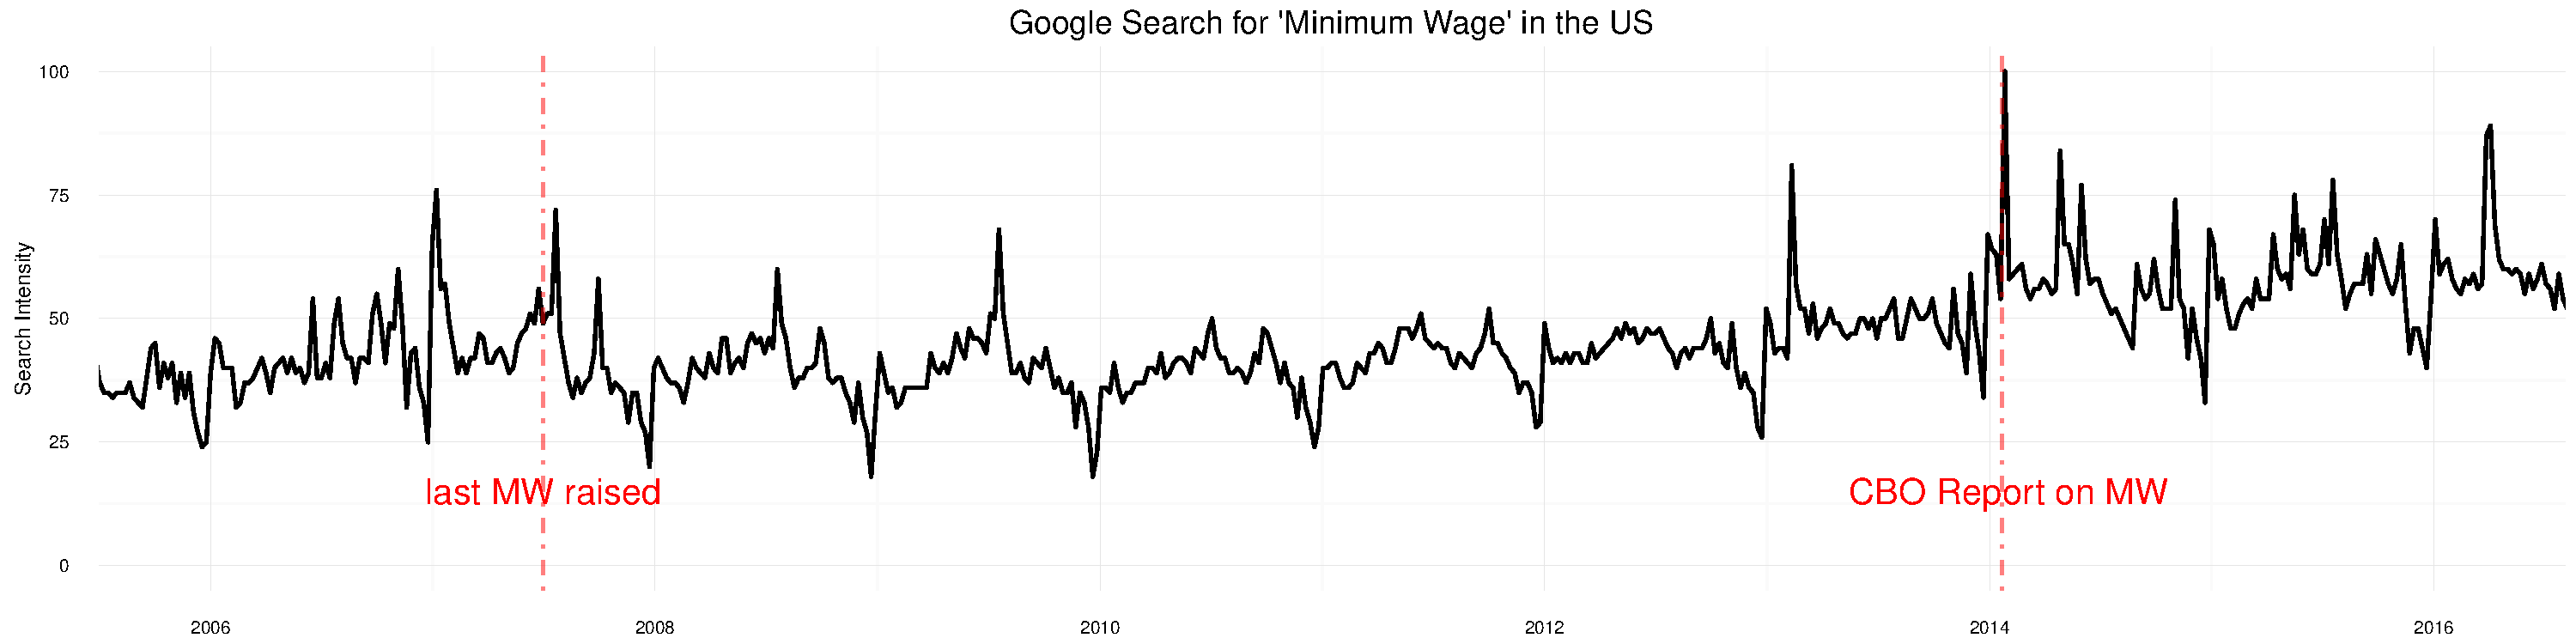
\includegraphics[scale = 0.22]{../Images/min_wage_gtrend}
\vspace*{-0.8em}
\caption{Google Search Intensity of ``Minimum Wage''}
\label{mw_gtrend}
\end{figure}	

\end{frame}

\section{Guidelines}

%6mins
\begin{frame}[shrink=25, label = pa_comp]{Guidelines Goal: Reproducibility \&  Transparency}

\tikzstyle{estimate} = [diamond, draw, node distance= 7em,text width = 5em, minimum height=5em, minimum width=5em, align = center]
\tikzstyle{line} = [draw, -stealth]
\tikzstyle{line_enph} = [draw, red, ultra thick]
\tikzstyle{inp} = [draw, rectangle, text centered, minimum height=3em, text width=2em, node distance= 2em]
\tikzstyle{source} = [draw, rectangle, text centered, minimum height=8em, text width=5em, node distance= 10em]
\tikzstyle{model} = [draw, rectangle, text centered, minimum height=8em, text width=15em, node distance= 10em]
%\tikzstyle{outp} = [draw, ellipse, text centered, minimum height=2mm, text width=2em, node distance= 10em]
%\tikzstyle{block} = [draw, rectangle,  text width=8em, text centered, minimum height=55mm, node distance= 5em]


%\begin{adjustbox}{max totalsize={1\textwidth}{.8\textheight},center}

\begin{figure}[h!]\centering 
\hspace*{-2.5em}
\begin{tikzpicture}[thick,scale=0.6, every node/.style={scale=0.6}]
\setbeamercovered{invisible}

%%%%%Nodes: Sources%%%%%%%
\onslide<1-5>\node [source](D_1){$Data$};
\onslide<1>\node [source, below = 1em of D_1](Lit){$Research$};
\onslide<1-5>\node [source, below = 1em of Lit](OR){\textit{Guess work}};


\draw[decoration={brace,mirror}, decorate] (-1.2,-10) -- node[below=6pt] {$Sources$}(1.1,-10);

\draw[decoration={brace,mirror}, decorate] (4.8,-11.3) -- node[below=6pt] {$Inputs$}(6.2,-11.3);


%node[below = 1em ](OR) -- node[below = 6em]{asd}(OR)


%\onslide<2-5>\node [source, color=red](Lit){$Research$};
\onslide<2-5>\node [source, below = 1em of D_1, color=red](Lit){$Research$};

%%%%%Nodes: Inputs%%%%%%%
\onslide<1-5>\node [inp, above right = 1em and 6em of  D_1 ](I_1){$I_1$};
\onslide<1-5>\node [inp, below = 1em of I_1](I_2){$I_2$};
\onslide<1-2>\node [inp, below = 8em of I_2](I_j){$I_j$};
\onslide<1-5>\node [inp, below right = 1em and 6em of OR ](I_last){$I_J$};

\onslide<3->\node [inp,  color=red, below = 8em of I_2](I_j){$I_j$};


\onslide<1-5>\path (I_2) -- node[auto=false, rotate=90, anchor=north, outer sep=-0.5em]{\ldots} (I_j);
\onslide<1-5>\path (I_j) -- node[auto=false, rotate=90, anchor=north, outer sep=-0.5em]{\ldots} (I_last);

%%%%%Paths connecting Sources with Inputs%%%%%%%
\onslide<1-5>\draw [line](D_1.east) -- (I_1.west);
\onslide<1-5>\draw [line](D_1.east) -- (I_2.west);
\onslide<1-2>\draw [line, opacity=1, anchor=center](Lit.east) -- (I_j.west);
\onslide<1-5>\draw [line, opacity=1, anchor=center](OR.east) -- (I_last.west);

\onslide<3->\draw [line,  color=red](Lit.east) -- (I_j.west);


\onslide<1-5>\draw [line, opacity=.3][xshift=1em](D_1.east) -- ([yshift=-8 em]I_1.west);
\onslide<1-5>\draw [line, opacity=.3][xshift=1em](D_1.east) -- ([yshift=-10 em]I_1.west);

\onslide<1-5>\draw [line, opacity=.3][xshift=1em](Lit.east) -- ([yshift=7 em]I_j.west);
\onslide<1-5>\draw [line, opacity=.3][xshift=1em](Lit.east) -- ([yshift=-5 em]I_j.west);

\onslide<1-5>\draw [line, opacity=.3][xshift=1em](OR.east) -- ([yshift=3 em]I_last.west);
\onslide<1-5>\draw [line, opacity=.3][xshift=1em](OR.east) -- ([yshift=5 em]I_last.west);


%%%%%Node and paths for model%%%%%%%
\onslide<1-3>\node [model, below right = 2em and 10em of D_1](model){$Model$};
\onslide<1-5>\draw [line](I_1) -| (model);
\onslide<1-5>\draw [line](I_2) -| (model);
\onslide<1-3>\draw [line](I_j) |- (model);
\onslide<1-5>\draw [line](I_last) -| (model);

\onslide<4->\node [model,  color=red, below right = 2em and 10em of D_1](model){$Model$};
\onslide<4->\draw [line,  color=red](I_j) |- (model);


%%%%%Node and paths for policy estimates%%%%%%%
\onslide<1-4>\node [estimate, right = 5em of model](PE_2){$Policy$ $Estimate_2$};
\onslide<1-4>\node [estimate, above = 5em of PE_2](PE_1){$Policy$ $Estimate_1$};
\onslide<1-4>\node [estimate, below = 5em of PE_2](PE_3){$Policy$ $Estimate_3$};


\onslide<1-4>\draw [line] (model.east) -- (PE_1.south west);
\onslide<1-4>\draw [line] (model.east) -- (PE_2.west);
\onslide<1-4>\draw [line] (model.east) -- (PE_3.north west);


\onslide<5->\node [estimate,  color=red, right = 5em of model](PE_2){$Policy$ $Estimate_2$};
\onslide<5->\node [estimate,  color=red, above = 5em of PE_2](PE_1){$Policy$ $Estimate_1$};
\onslide<5->\node [estimate,  color=red, below = 5em of PE_2](PE_3){$Policy$ $Estimate_3$};


\onslide<5->\draw [line,  color=red] (model.east) -- (PE_1.south west);
\onslide<5->\draw [line,  color=red] (model.east) -- (PE_2.west);
\onslide<5->\draw [line,  color=red] (model.east) -- (PE_3.north west);
\end{tikzpicture}
\end{figure}

\end{frame}





\begin{frame}{Summary of Adapted Guidelines}
 \centering
 \resizebox{25em}{10em}{%
    \begin{tabular}{ P{1.2cm} P{1.5cm} P{3cm}  P{3cm}  P{3cm} }
     \toprule
     {\black Standard} & {\black Level 0} 	& {\black Level 1} & {\black Level 2} & {\black Level 3} \\
     \midrule      \midrule
   {\black Workflow} & {\gray Policy estimates vaguely described}  & {\gray All the inputs, and their corresponding sources, used in the calculations are listed } & {\gray Lvl 1 + Policy estimates are listed, in same unit if possible} & {\gray Lvl 2 + all the components can be modified with little effort} \\
     \midrule
    {\black Data} & {\gray Report says nothing} & {\gray Clearly stated whether all, some components, or none of the data is available, with instructions for access when possible.} & {\gray Lvl 1 + report and data are in same place} & {\gray Lvl 2 + Report has specific lines of code that call the data and changes in the data produce traceable changes in the report} \\
     \midrule
      {\black Methods \& Code} & {\gray Key assumption are listed} & {\gray Methods are described in prose. Large amount of work is required to reproduce qualitatively similar estimates}  & {\gray Methods and described in prose, with detailed formulas, and code is provided as supplementary material} & {\gray Lvl 2 + All is in the same document where changes in the code affect the output automatically} \\
     \toprule
     \multicolumn{5}{ P{11.7cm} }{  \raggedleft {\black\small{ From TOP guidelines \citep{nosek2015promoting} v1.0.1}} \small{\hyperlink{no_gray}{\beamerbutton{}}} }
   \end{tabular}}
\end{frame}


\begin{frame}[noframenumbering]{Summary of Adapted Guidelines}
 \centering
 \resizebox{25em}{10em}{%
    \begin{tabular}{ P{1.2cm} P{1.5cm} P{3cm}  P{3cm}  P{3cm} }
     \toprule
    {\black Standard} & {\red Level 0 } 	&  {\red Level 1 } &  {\red Level 2}  & {\red Level 3 }  \\
     \midrule      \midrule
    {\black Workflow} & {\gray Policy estimates vaguely described}  & {\gray All the inputs, and their corresponding sources, used in the calculations are listed } & {\gray Lvl 1 + Policy estimates are listed, in same unit if possible} & {\gray Lvl 2 + all the components can be modified with little effort} \\
     \midrule
    {\black Data} & {\gray Report says nothing} & {\gray Clearly stated whether all, some components, or none of the data is available, with instructions for access when possible.} & {\gray Lvl 1 + report and data are in same place} & {\gray Lvl 2 + Report has specific lines of code that call the data and changes in the data produce traceable changes in the report} \\
     \midrule
      {\black Methods \& Code} & {\gray Key assumption are listed} & {\gray Methods are described in prose. Large amount of work is required to reproduce qualitatively similar estimates}  & {\gray Methods and described in prose, with detailed formulas, and code is provided as supplementary material} & {\gray Lvl 2 + All is in the same document where changes in the code affect the output automatically} \\
     \toprule
     \multicolumn{5}{ P{11.7cm} }{  \raggedleft {\black\small{ From TOP guidelines \citep{nosek2015promoting} v1.0.1}} \small{\hyperlink{no_gray}{\beamerbutton{}}} }
   \end{tabular}}
\end{frame}


\begin{frame}[noframenumbering]{Summary of Adapted Guidelines}
 \centering
 \resizebox{25em}{10em}{%
    \begin{tabular}{ P{1.2cm} P{1.5cm} P{3cm}  P{3cm}  P{3cm} }
     \toprule
     {\red Standard} & {\black Level 0} 	& {\black Level 1} & {\black Level 2} & {\black Level 3} \\
     \midrule      \midrule
    {\red Workflow} & {\gray Policy estimates vaguely described}  & {\gray All the inputs, and their corresponding sources, used in the calculations are listed} & {\gray Lvl 1 + Policy estimates are listed, in same unit if possible} & {\gray Lvl 2 + all the components can be modified with little effort} \\
     \midrule
    {\red Data} & {\gray Report says nothing} & {\gray Clearly stated whether all, some components, or none of the data is available, with instructions for access when possible.} & {\gray Lvl 1 + report and data are in same place} & {\gray Lvl 2 + Report has specific lines of code that call the data and changes in the data produce traceable changes in the report} \\
     \midrule
      {\red Methods \& Code} & {\gray Key assumption are listed} & {\gray Methods are described in prose. Large amount of work is required to reproduce qualitatively similar estimates}  & {\gray Methods and described in prose, with detailed formulas, and code is provided as supplementary material} & {\gray Lvl 2 + All is in the same document where changes in the code affect the output automatically} \\
     \toprule
     \multicolumn{5}{ P{11.7cm} }{  \raggedleft {\black\small{ From TOP guidelines \citep{nosek2015promoting} v1.0.1}} \small{\hyperlink{no_gray}{\beamerbutton{}}} }
   \end{tabular}}
\end{frame}

\begin{frame}[noframenumbering, label=guidelines_sum]{Summary of Adapted Guidelines}
 \centering
 \resizebox{25em}{10em}{%
    \begin{tabular}{ P{1.2cm} P{1.5cm} P{3cm}  P{3cm}  P{3cm} }
     \toprule
     Standard & Level 0 	& Level 1 & Level 2 & Level 3 \\
     \midrule      \midrule
   {\black Workflow} & {\gray Policy estimates vaguely described}  & {\gray All the inputs, and their corresponding sources, used in the calculations are listed } & {\gray Lvl 1 + Policy estimates are listed, in same unit if possible} & {\gray Lvl 2 + all the components can be modified with little effort} \\
     \midrule
    {\black Data} & {\gray Report says nothing} & {\gray Clearly stated whether all, some components, or none of the data is available, with instructions for access when possible.} & {\gray Lvl 1 + report and data are in same place} & {\gray Lvl 2 + Report has specific lines of code that call the data and changes in the data produce traceable changes in the report} \\
     \midrule
      {\black Methods \& Code} & {\gray Key assumption are listed} & {\gray Methods are described in prose. Large amount of work is required to reproduce qualitatively similar estimates}  & {\gray Methods and described in prose, with detailed formulas, and code is provided as supplementary material} & {\gray Lvl 2 + All is in the same document where changes in the code affect the output automatically} \\
     \toprule
     \multicolumn{5}{ P{11.7cm} }{  \raggedleft {\red\small{ From TOP guidelines \citep{nosek2015promoting} v1.0.1}} \small{\hyperlink{no_gray}{\beamerbutton{}}} }
   \end{tabular}}
\end{frame}

\section{Application}


\begin{frame}[label=fr_pa]{\textbf{Before: } Applying Guidelines to CBO Report}
 \centering
 \resizebox{25em}{10em}{%
    \begin{tabular}{ P{1.2cm} P{1.5cm} P{3cm}  P{3cm}  P{3cm} }
     \toprule
     Standard & Level 0 	& Level 1 & Level 2 & Level 3 \\
     \midrule      \midrule
    Workflow &  Policy estimates vaguely described  &  All the inputs, and their corresponding sources, used in the calculations are listed & {\gray Lvl 1 + Policy estimates are listed, in same unit if possible} & {\gray Lvl 2 + all the components can be modified with little effort} \\
     \midrule
    Data & Report says nothing & Clearly stated whether all, some components, or none of the data is available, with instructions for access when possible. & {\gray Lvl 1 + report and data are in same place} & {\gray Lvl 2 + Report has specific lines of code that call the data and changes in the data produce traceable changes in the report} \\
     \midrule
      Methods \& Code &  Key assumption are listed & Methods are described in prose. Large amount of work is required to reproduce qualitatively similar estimates & {\gray Methods and described in prose, with detailed formulas, and code is provided as supplementary material} & {\gray Lvl 2 + All is in the same document where changes in the code affect the output automatically} \\
     \toprule
     \multicolumn{5}{ P{11.7cm} }{ \raggedleft \small{ From TOP guidelines \citep{nosek2015promoting} v1.0.1} \small{\hyperlink{low_tr_ex}{\beamerbutton{}}}  }
   \end{tabular}
   }
\end{frame}







\begin{frame}[label=demo]{\textbf{After: } Applying Guidelines to Build Dynamic Document}
\begin{center}

{\Huge
\texttt{\href{https://rpubs.com/fhoces/dd_cbo_mw}{{\blue\underline{DEMO}}}}
}\small{\hyperlink{no_inet}{\beamerbutton{}}}


\end{center}

%Discuss automation 

\end{frame}



\begin{frame}[shrink=25, label=map_cbo]{Benefit 1: Map the complete policy analysis}

\tikzstyle{estimate} = [diamond, draw, node distance= 7em,text width = 5em, minimum height=5em, minimum width=5em, align = center]
\tikzstyle{line} = [draw, -stealth]
\tikzstyle{line_enph} = [draw, red, ultra thick]
\tikzstyle{inp} = [draw, rectangle, text centered, minimum height=3em, text width=2em, node distance= 2em]
\tikzstyle{source} = [draw, rectangle, text centered, minimum height=8em, text width=5em, node distance= 10em]
\tikzstyle{model} = [draw, rectangle, text centered, minimum height=8em, text width=15em, node distance= 10em]
%\tikzstyle{outp} = [draw, ellipse, text centered, minimum height=2mm, text width=2em, node distance= 10em]
%\tikzstyle{block} = [draw, rectangle,  text width=8em, text centered, minimum height=55mm, node distance= 5em]


\begin{figure}[h!]\centering \label{pa_components_ex}
\hspace*{-2.5em}
\begin{tikzpicture}[thick,scale=0.6, every node/.style={scale=0.6}]
\setbeamercovered{invisible}

%%%%%Nodes: Sources%%%%%%%
\node [source](D_1){CPS ORG; CPS ASEC; CBO 10-Y projections};
\node [source, below = 1em of D_1](Lit){Labor demand for teenagers; Ripple effects};
\node [source, below = 1em of Lit](OR){Extrapolation for adults; Aggregate effects; Dist of losses};


\draw[decoration={brace,mirror}, decorate] (-1.2,-10) -- node[below=6pt] {$Sources$}(1.1,-10);

\draw[decoration={brace,mirror}, decorate] (4.8,-11.3) -- node[below=6pt] {$Inputs$}(6.2,-11.3);


%node[below = 1em ](OR) -- node[below = 6em]{asd}(OR)



%%%%%Nodes: Inputs%%%%%%%
\node [inp, above right = 1em and 6em of  D_1 ](I_1){$dF_{w}$};
\node [inp, below = 1em of I_1](I_2){$g_{N}$};
\node [inp, below = 10em of I_2](I_j){$\eta_{teens}$};
\node [inp, below right = 1em and 6em of OR ](I_last){$F_{ext}$};



\path (I_2) -- node[auto=false, rotate=90, anchor=north, outer sep=-0.5em]{\ldots} (I_j);
\path (I_j) -- node[auto=false, rotate=90, anchor=north, outer sep=-0.5em]{\ldots} (I_last);

%%%%%Paths connecting Sources with Inputs%%%%%%%
\draw [line](D_1.east) -- (I_1.west);
\draw [line](D_1.east) -- (I_2.west);
\draw [line, opacity=1, anchor=center](Lit.east) -- (I_j.west);
\draw [line, opacity=1, anchor=center](OR.east) -- (I_last.west);

\draw [line, opacity=.3][xshift=1em](D_1.east) -- ([yshift=-8 em]I_1.west);
\draw [line, opacity=.3][xshift=1em](D_1.east) -- ([yshift=-10 em]I_1.west);

\draw [line, opacity=.3][xshift=1em](Lit.east) -- ([yshift=7 em]I_j.west);
\draw [line, opacity=.3][xshift=1em](Lit.east) -- ([yshift=-5 em]I_j.west);

\draw [line, opacity=.3][xshift=1em](OR.east) -- ([yshift=3 em]I_last.west);
\draw [line, opacity=.3][xshift=1em](OR.east) -- ([yshift=5 em]I_last.west);


%%%%%Node and paths for model%%%%%%%
\node [model, below right = 2em and 10em of D_1](model){\hyperlink{equations}{Equations}: \ref{N_final} - \ref{last.eq} };
\draw [line](I_1) -| (model);
\draw [line](I_2) -| (model);
\draw [line](I_j) |- (model);
\draw [line](I_last) -| (model);

%%%%%Node and paths for policy estimates%%%%%%%
\node [estimate, right = 5em of model](PE_2){Average wage gain};
\node [estimate, above = 5em of PE_2](PE_1){Average wage loss};
\node [estimate, below = 5em of PE_2](PE_3){Average balance loss};


\draw [line] (model.east) -- (PE_1.south west);
\draw [line] (model.east) -- (PE_2.west);
\draw [line] (model.east) -- (PE_3.north west);


\end{tikzpicture}
\end{figure}
\hyperlink{full_model}{\beamerbutton{}}
\hyperlink{equations}{\beamerbutton{}}
\end{frame}

\begin{frame}[label=low_tr_ex]{Benefit 2: Easier Methodological Appraisal. Example: dis-employment effects \textbf{Before}}


Steps taken to verify the analysis \&  employment variation $(\widehat{\Delta E}\times 1000)$ at each line\footnotemark 

\footnotetext[1]{Assuming target population $\approx 22$ million, $\overline{\Delta w_{w\leq MW^{'}}} \approx 14\%$, and non-compliance $\approx 15\%$ }
 

\begin{enumerate}
\pause
\item Find an elasticity: -0.1 (page 25): {\red $\widehat{\Delta E} \approx 300$ }
\pause
\item What about adults? $\eta^{adults}=\frac{1}{3}\eta^{teens}$ (page 28):  {\red $\widehat{\Delta E} \approx 100$  } 
\pause
\item What about the adjustment? $\widetilde{ \eta^{g}_{w\leq MW} } =  \frac{\eta^{g}_{lit}}{p^{g}_{w\leq MW}} \times \frac{\%\Delta MW}{\overline{\%\Delta w^{g}}}$ (page 26-28 + 2 papers):   {\red $\widehat{\Delta E} \approx 1,100$  } 
\pause
\item The adjustment factors $\frac{1}{p^{g}_{w\leq MW}} \times \frac{\%\Delta MW}{\overline{\%\Delta w^{g}}} = F^{g}_{adj}$ are not computed from the data (3.2 teens, 19.5 adults). Instead: $F^{teen}_{adj} = F^{adult}_{adj}= 4.5$ (page 28) ${\red\widehat{\Delta E} \approx 500}$   
\end{enumerate}
\textit{Steps 2-4 took several days of work! }
\small{\hyperlink{fr_pa}{\beamerbutton{}}}
\end{frame}

\begin{frame}{Benefit 3: All in one Output 1/3}
\begin{figure}[h!]
\centering
\hspace*{-3em}
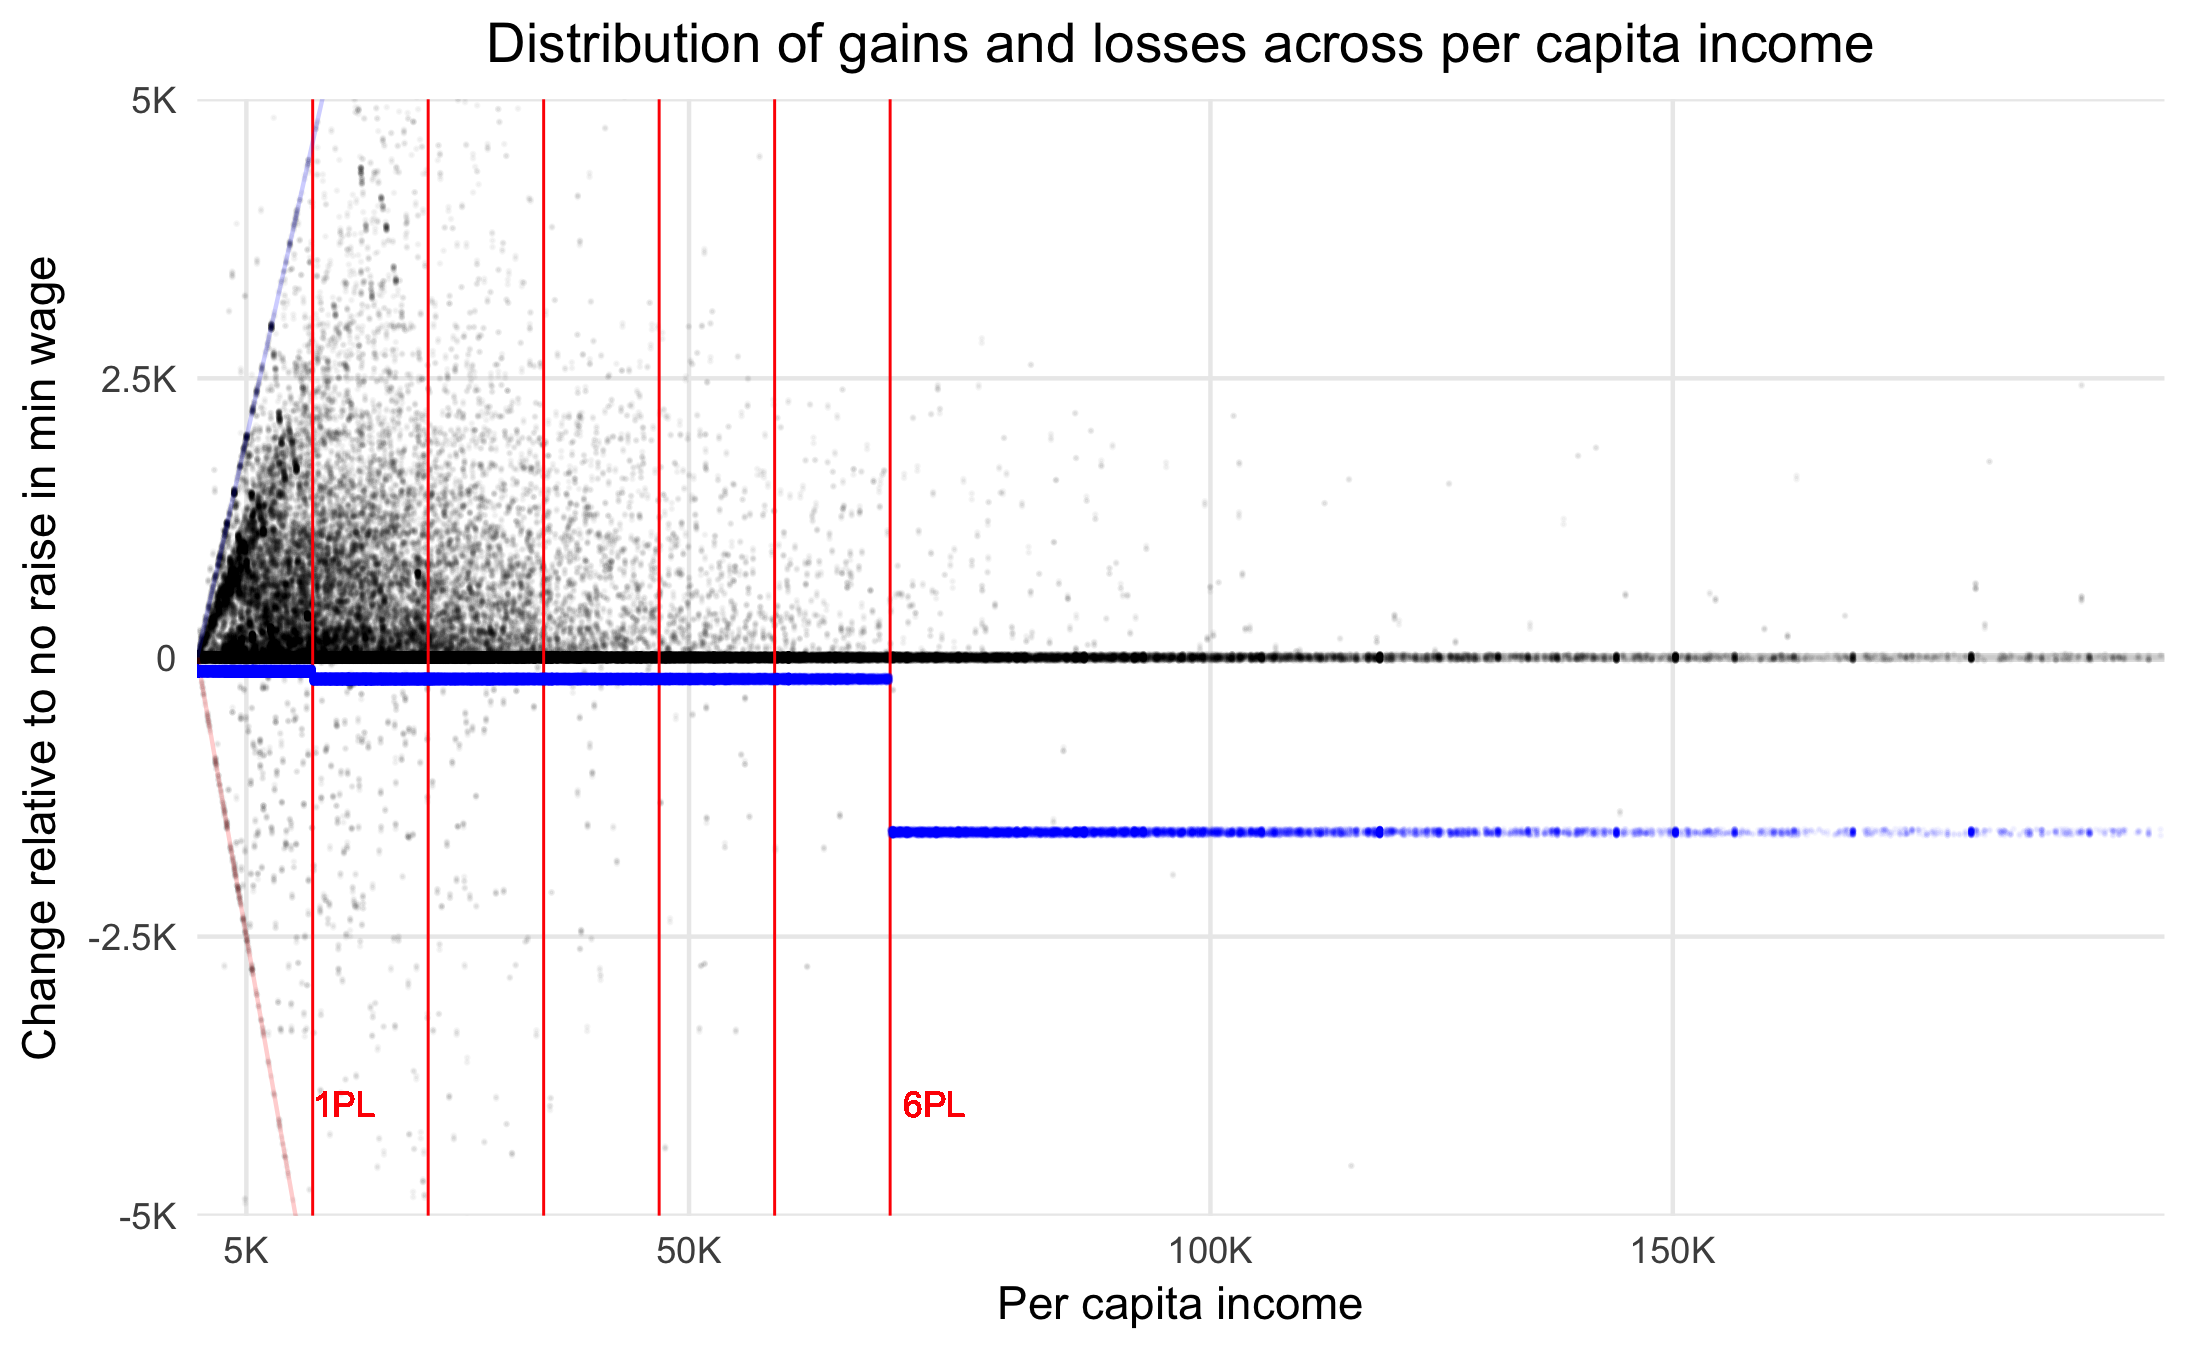
\includegraphics[scale = 0.13]{../Images/alt_pe1}
\caption{Gains and losses. Different Units}
\end{figure}	
\end{frame}

\begin{frame}{Benefit 3: All in one Output 2/3}
\begin{figure}[h!]
\centering
\hspace*{-3em}
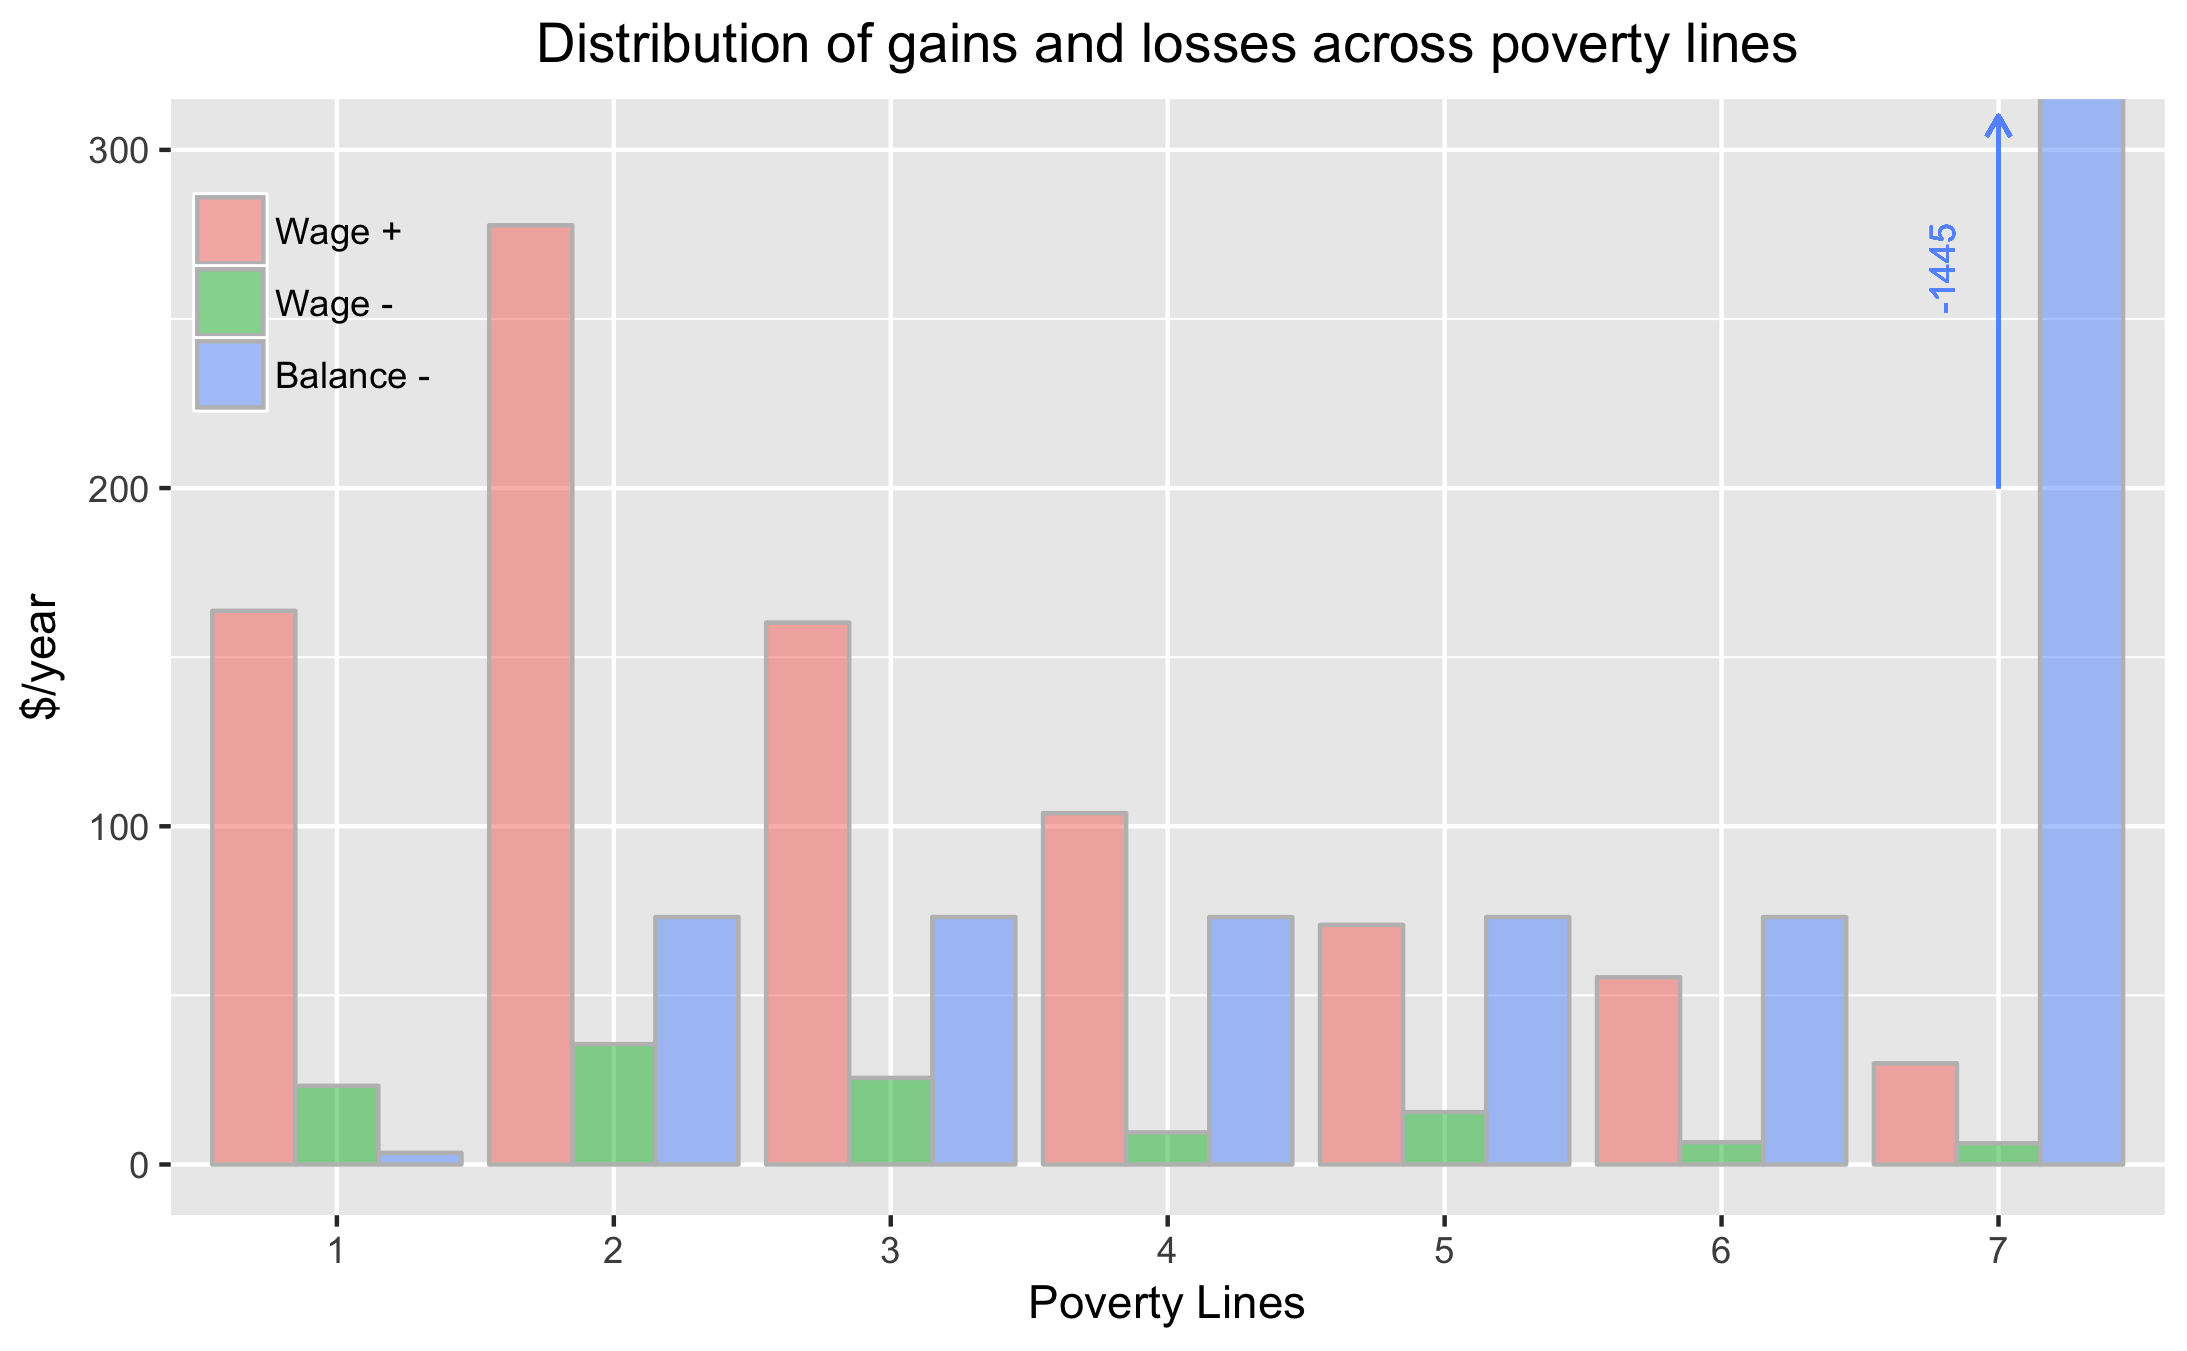
\includegraphics[scale = 0.13]{../Images/alt_pe2}
\caption{Gains and losses. Different Denominator}
\end{figure}	
\end{frame}

\begin{frame}{Benefit 3: All in one Output 3/3}
\begin{figure}[h!]
\centering
\hspace*{-3em}
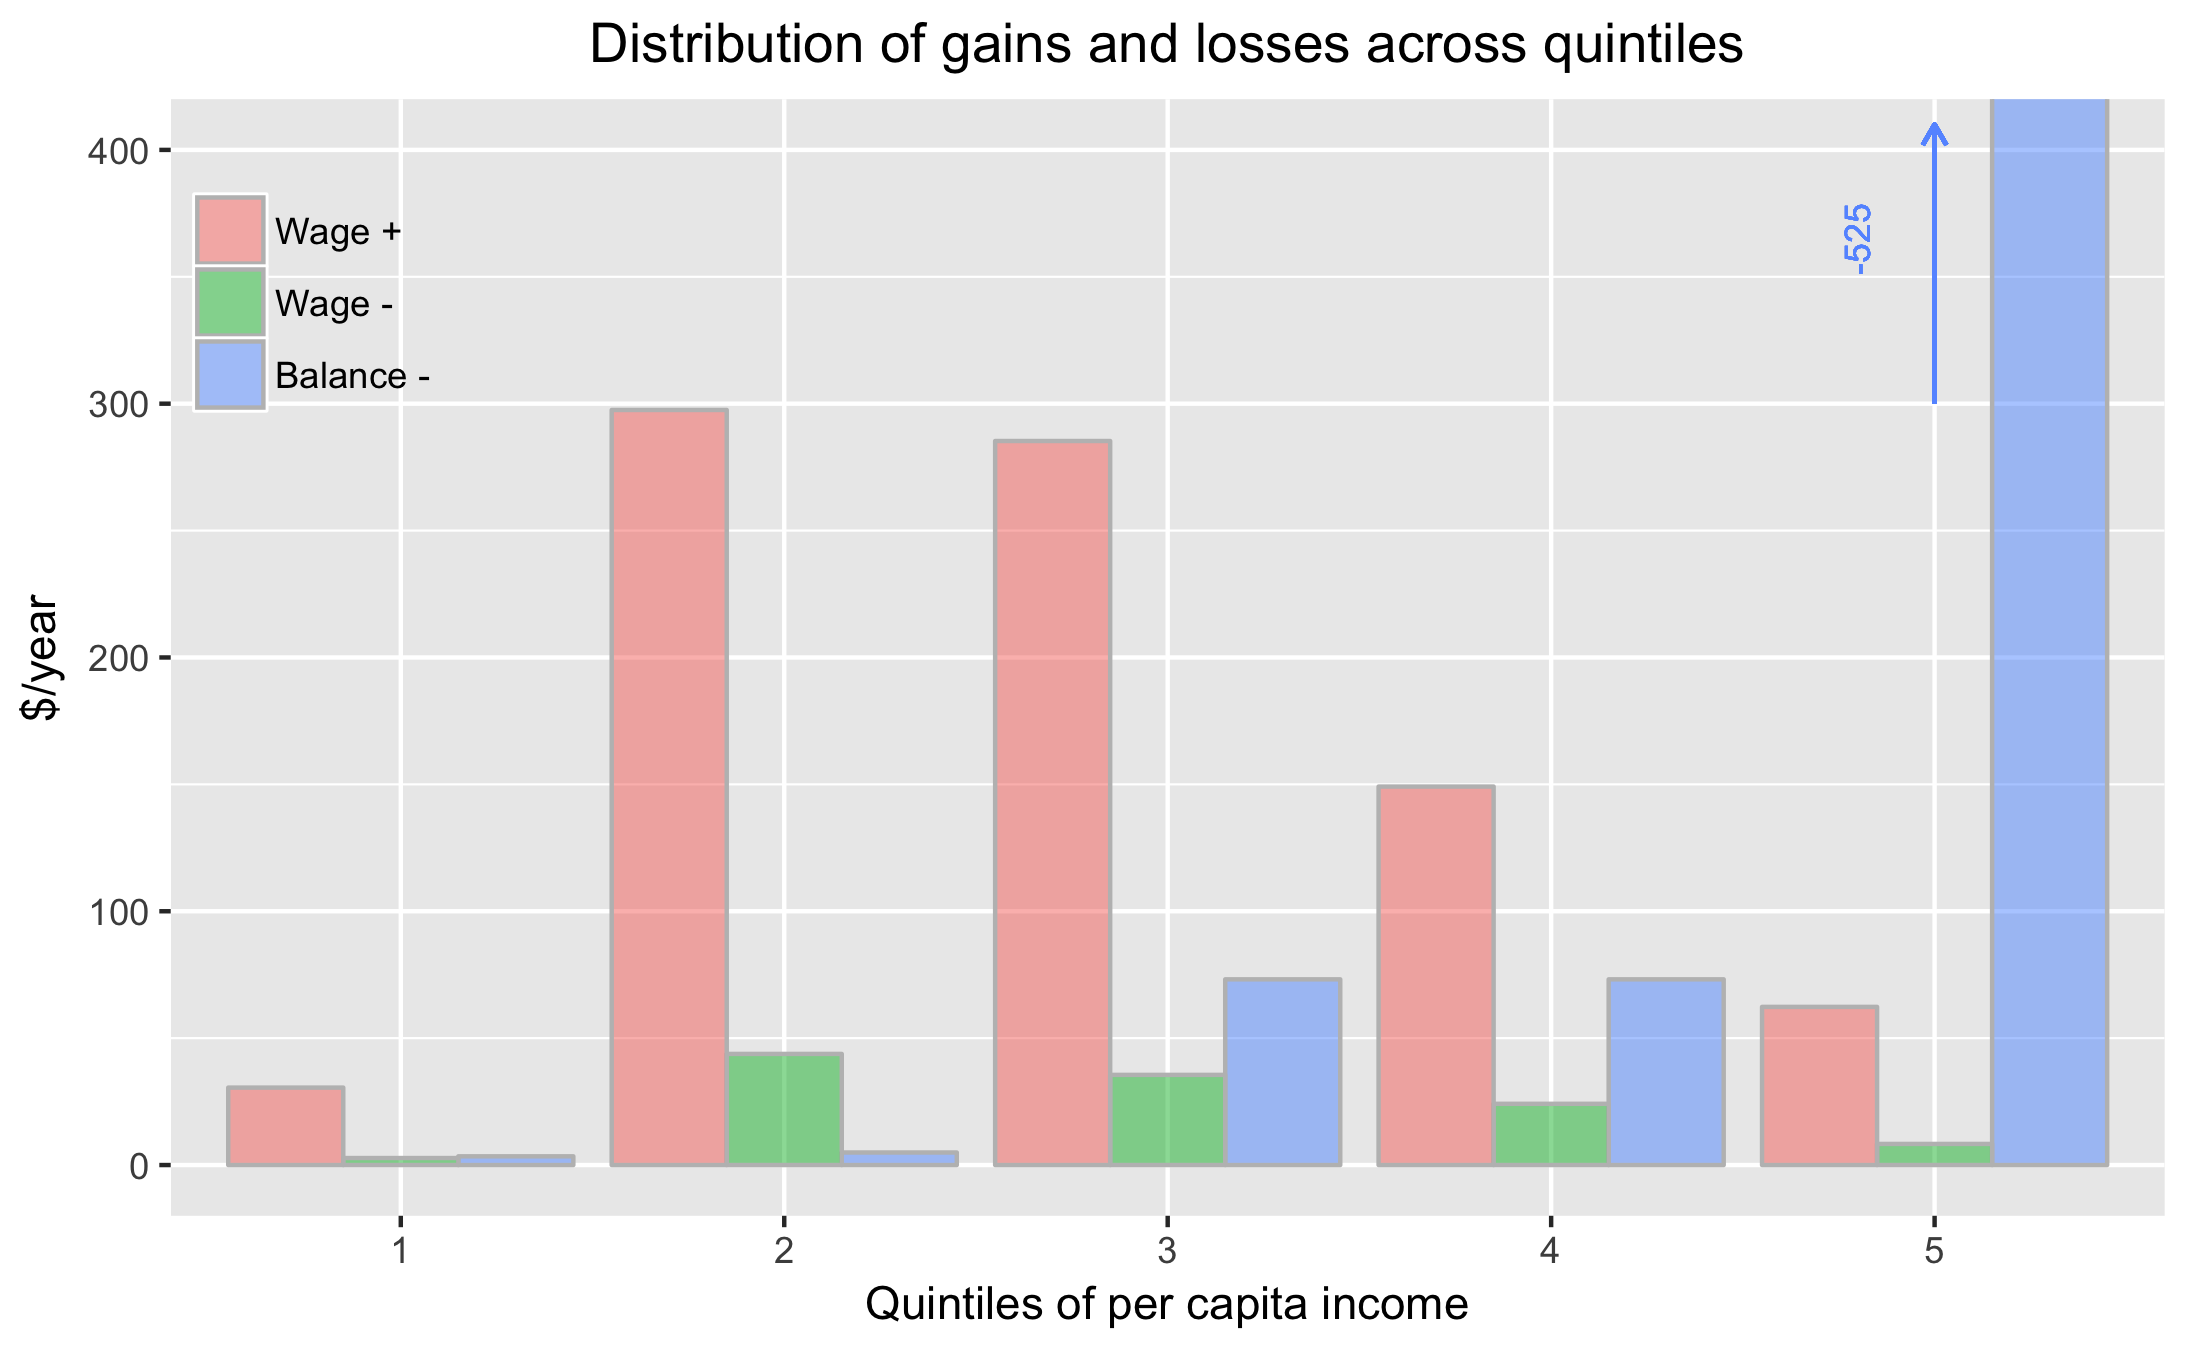
\includegraphics[scale = 0.13]{../Images/policy_est}
\caption{Gains and losses. Same units and denominator}
\end{figure}	
\end{frame}


\section{Sensitivity Analysis}

\begin{frame}[noframenumbering]{Sensitivity Analysis: Status Quo}
\begin{figure}[h!]
\centering
\hspace*{-3em}
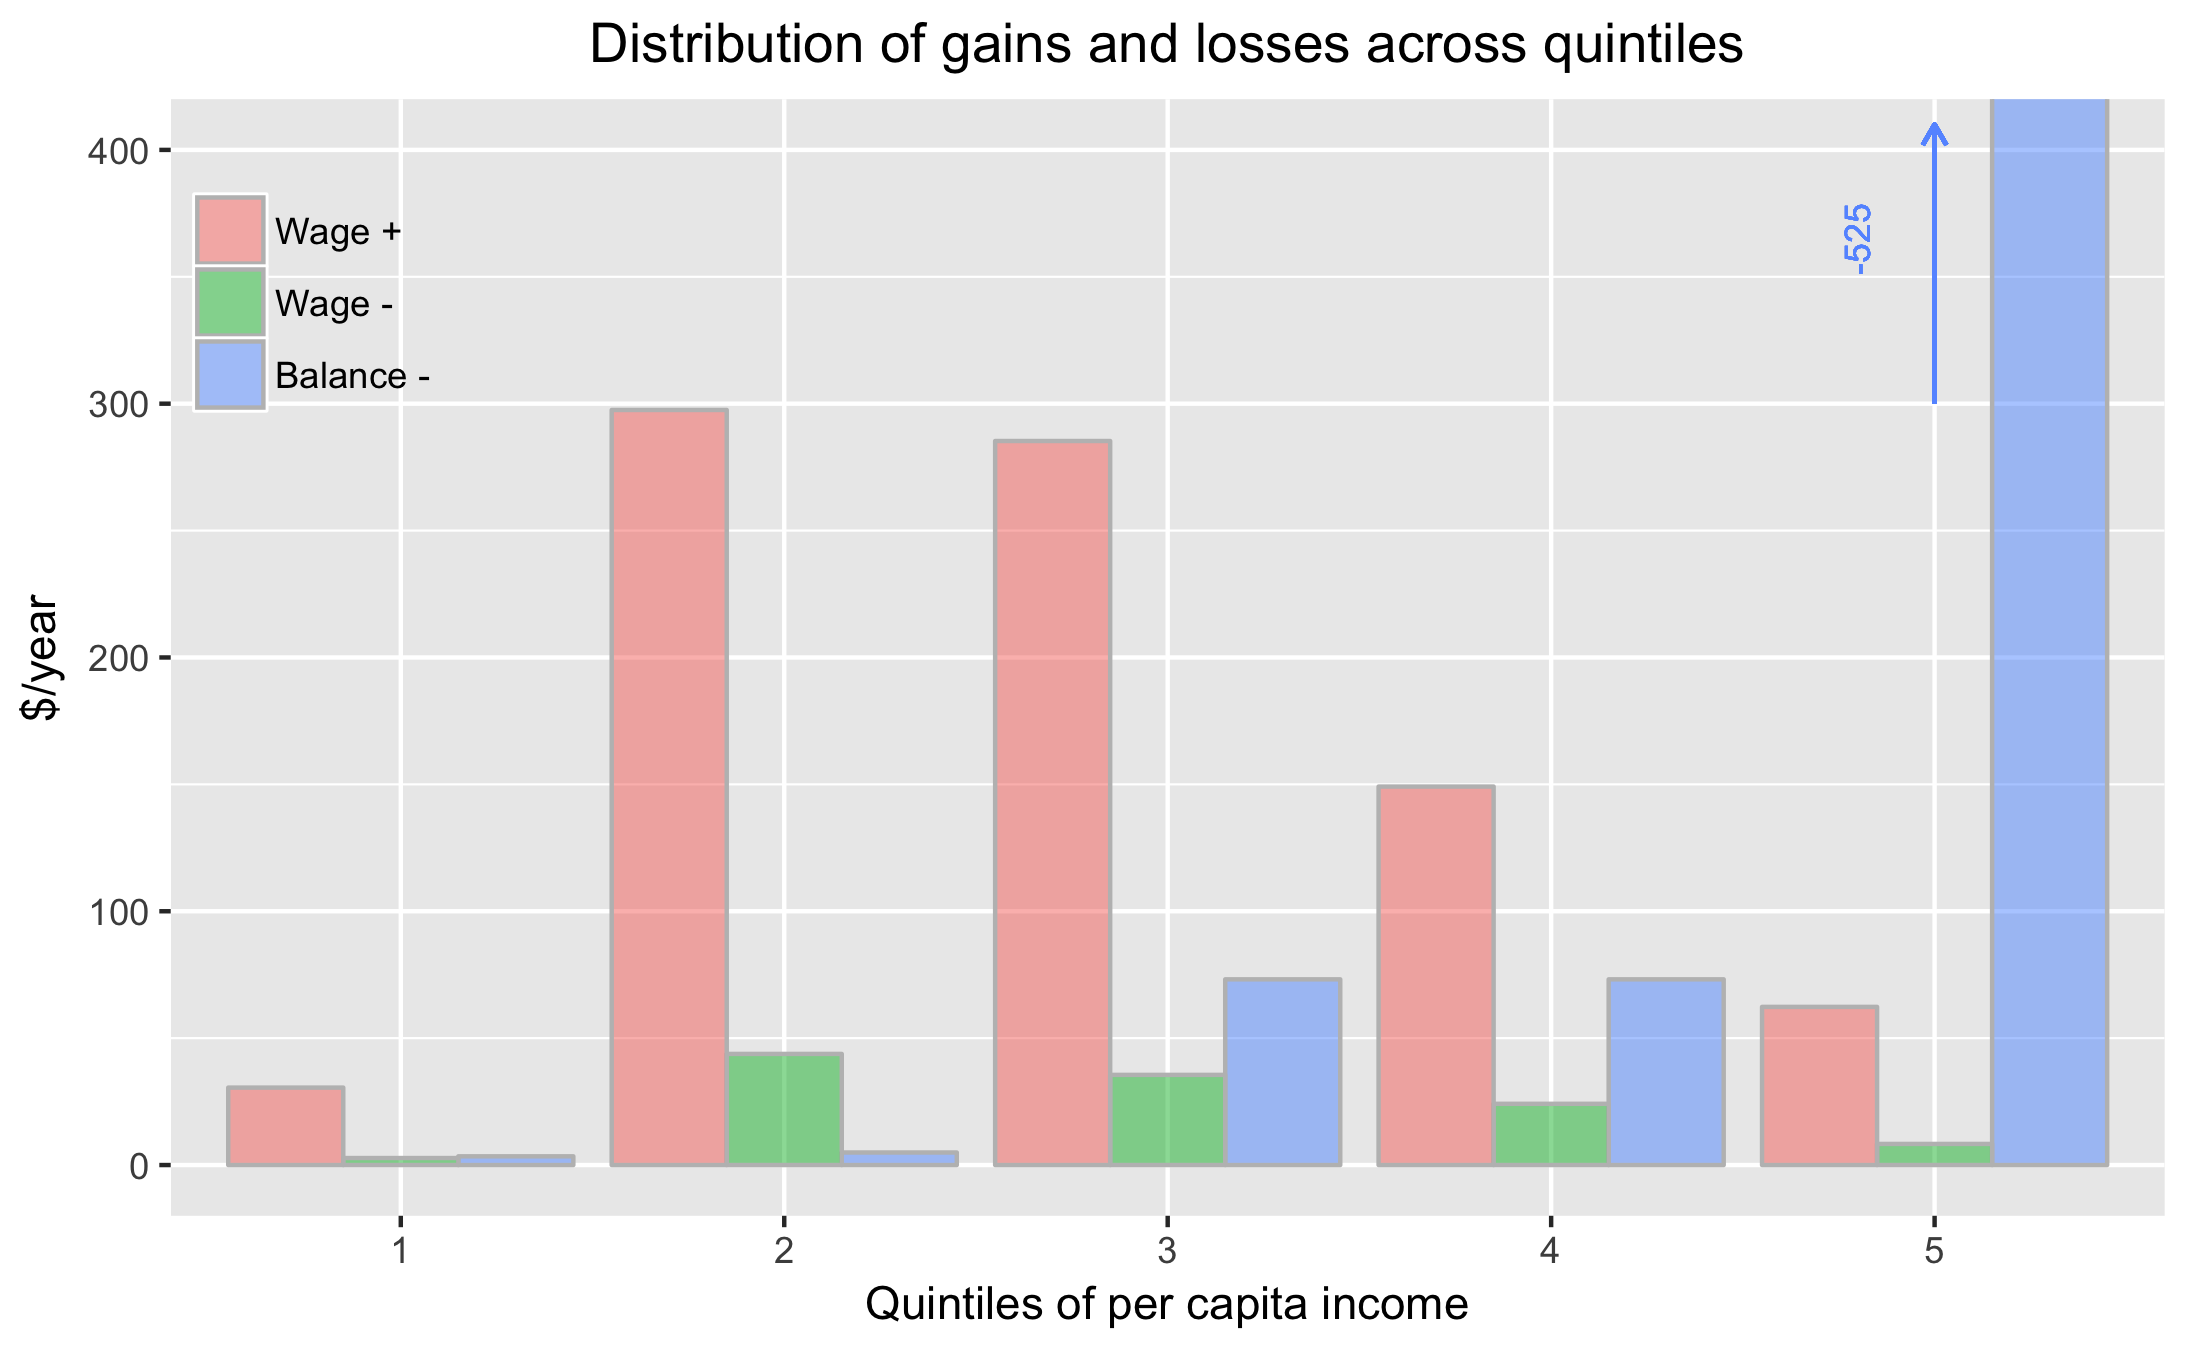
\includegraphics[scale = 0.13]{../Images/policy_est}
\caption{Default settings {\white $ \eta $} }
\end{figure}	
\end{frame}

\begin{frame}{SA: Change in Elasticity of Labor Demand}
\begin{figure}[h!]
\centering
\hspace*{-3em}
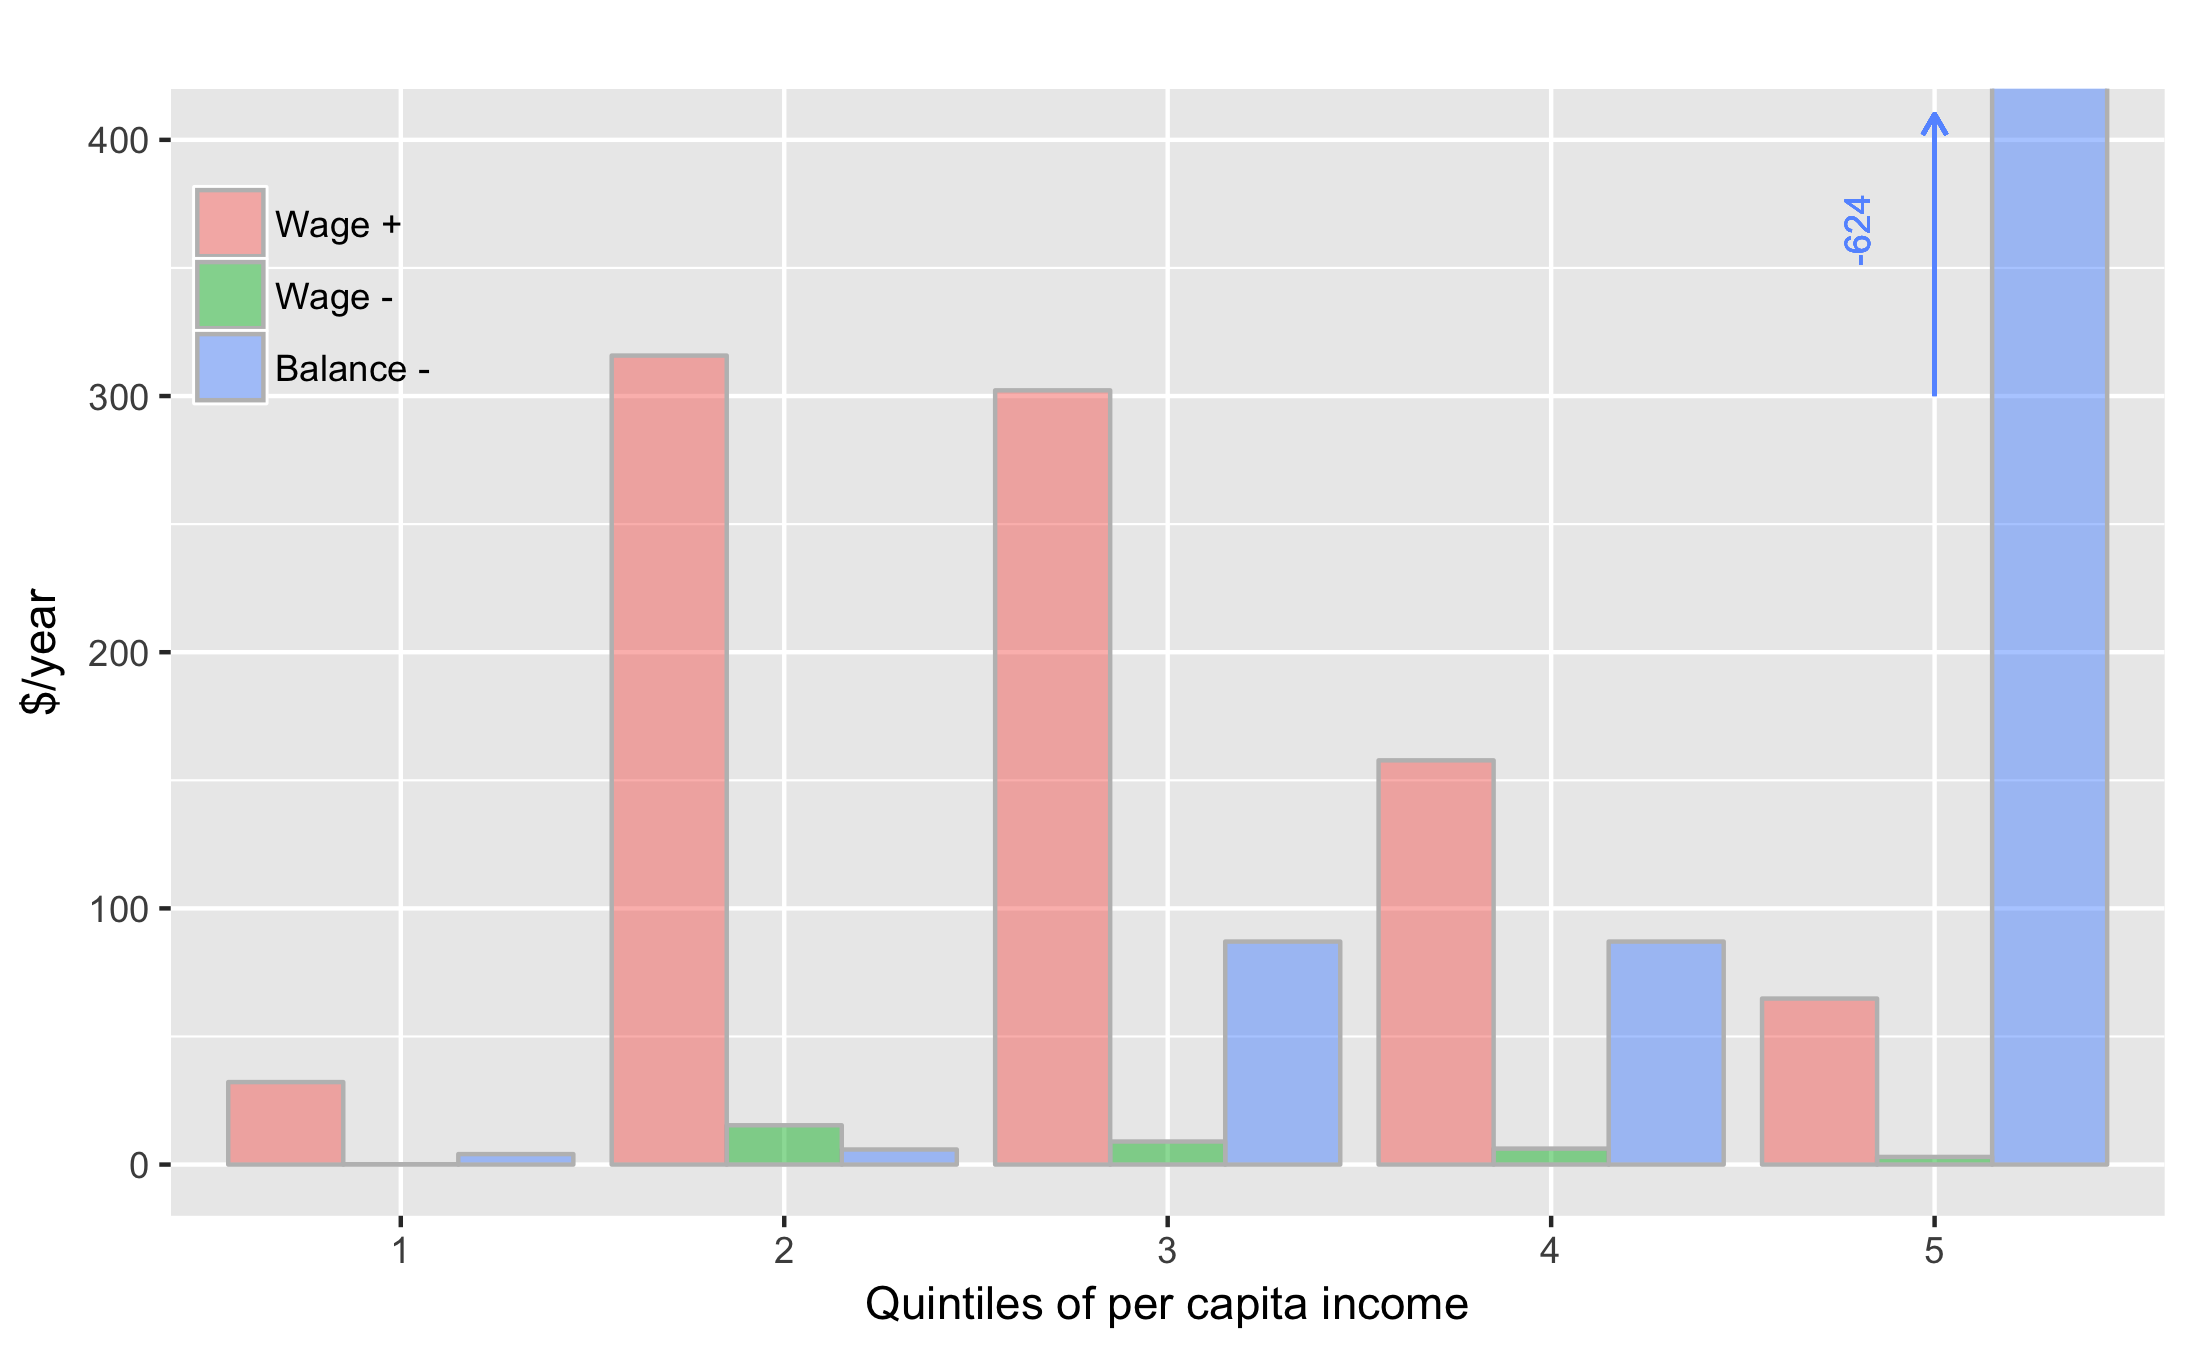
\includegraphics[scale = 0.13]{../Images/policy_est_eta001}
\caption{From $\eta^{teens}_{lit} = - 0.1$ to  $\eta^{teens}_{lit} = - 0.01(\Delta^{-}90\%)$}
\end{figure}	
\end{frame}

\begin{frame}[noframenumbering]{Sensitivity Analysis: Status Quo}
\begin{figure}[h!]
\centering
\hspace*{-3em}
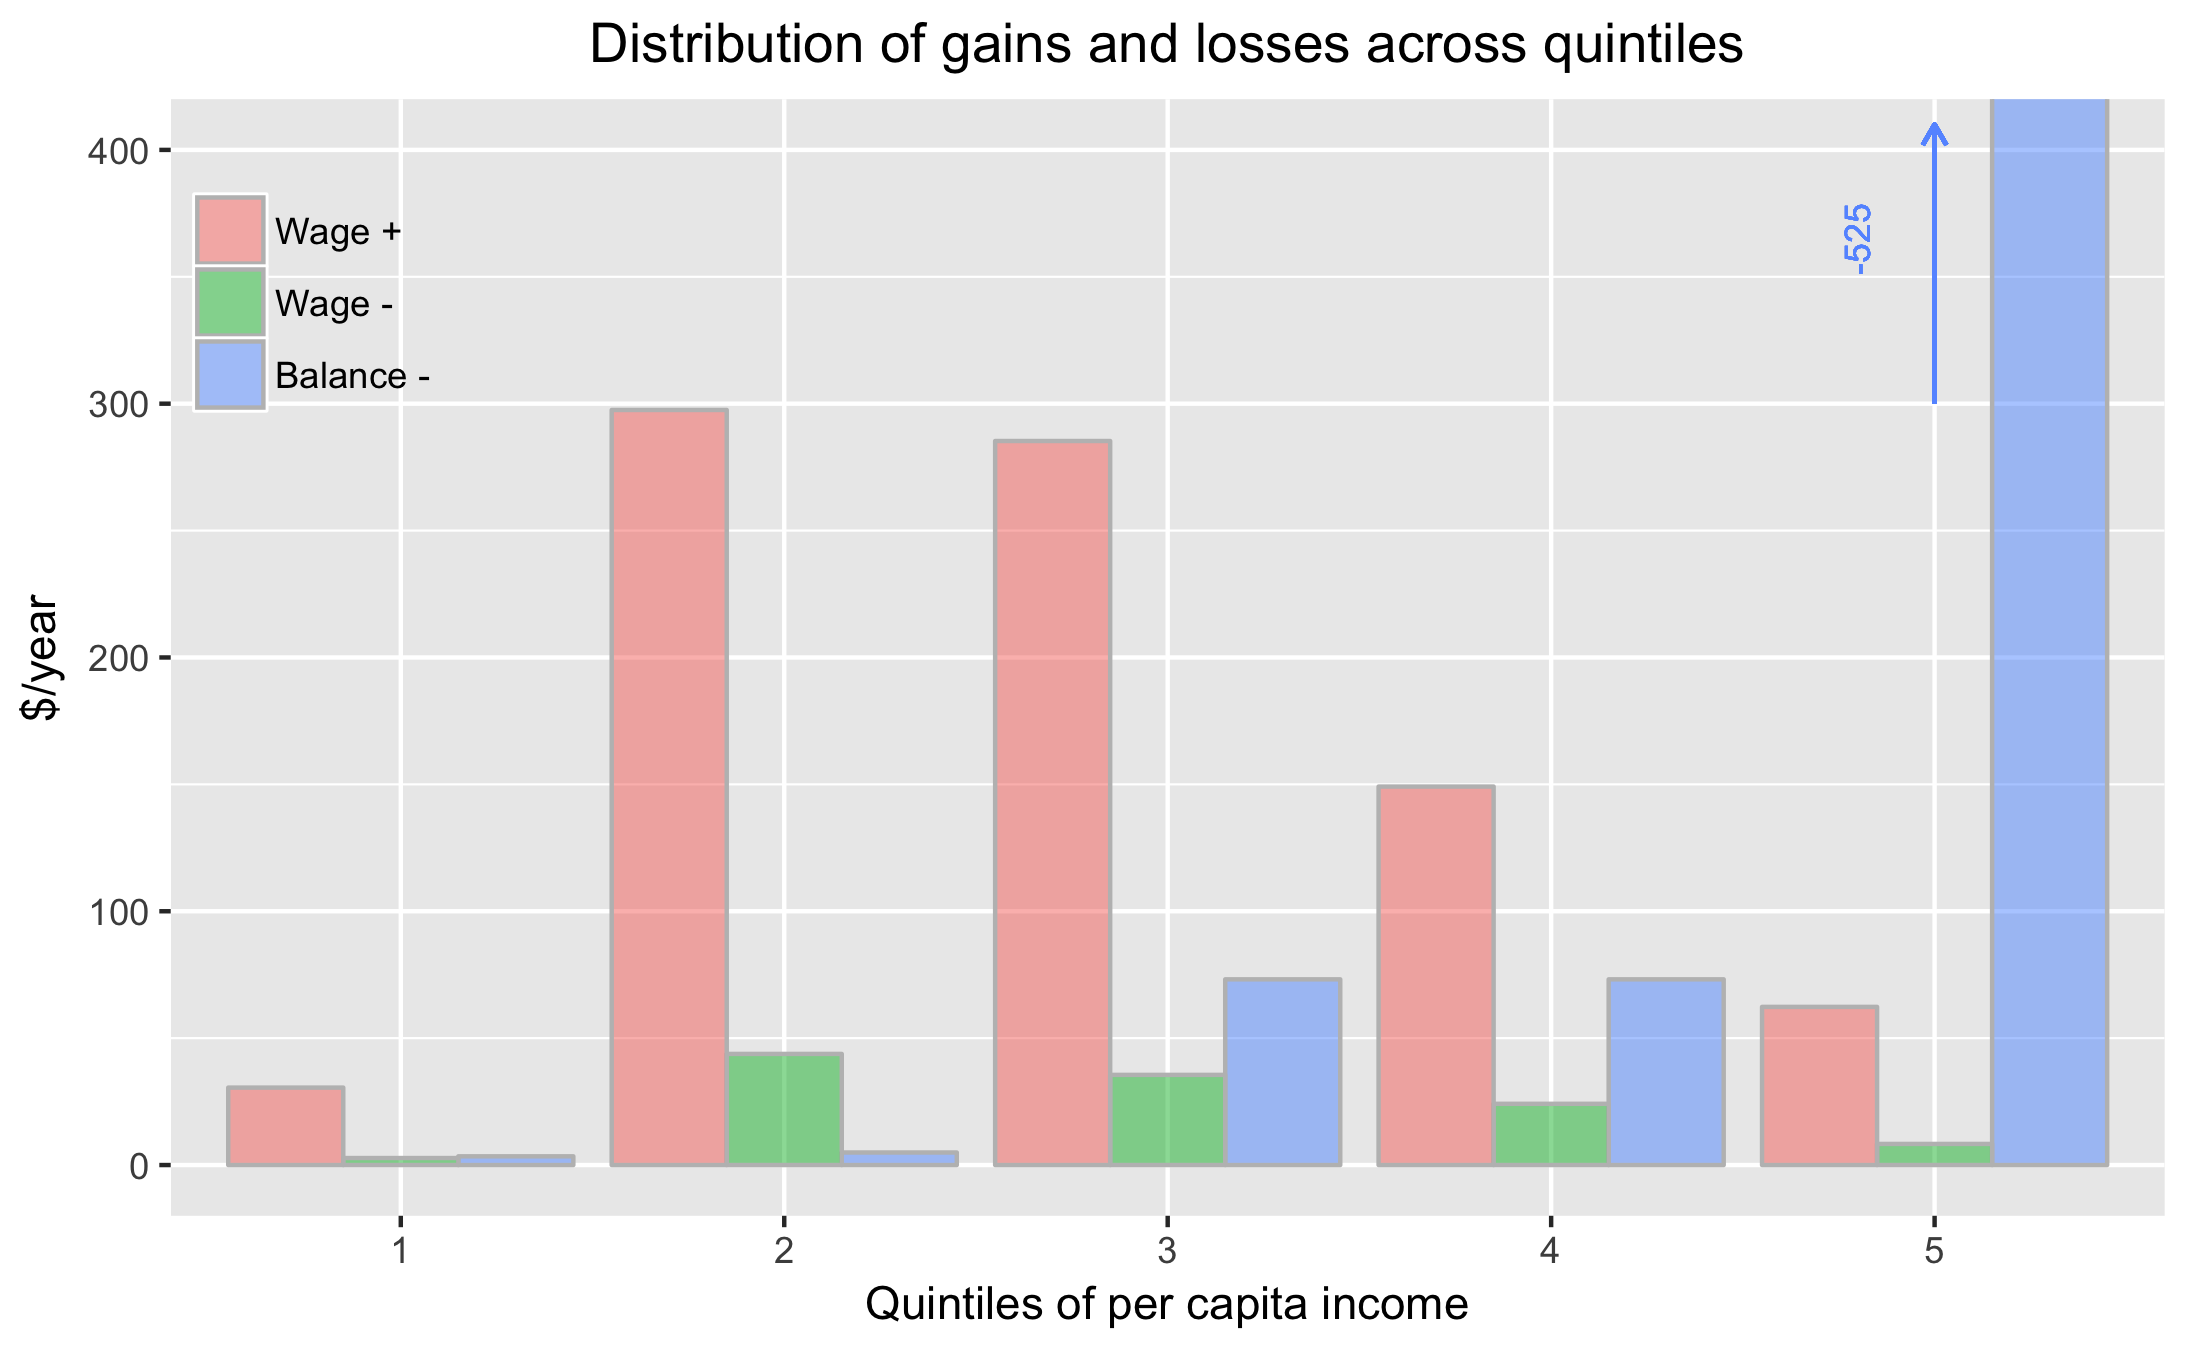
\includegraphics[scale = 0.13]{../Images/policy_est}
\caption{Default settings {\white $ \eta $} }
\end{figure}	
\end{frame}

\begin{frame}{SA: Change in Distribution of Balance Loses}
\begin{figure}[h!]
\centering
\hspace*{-3em}
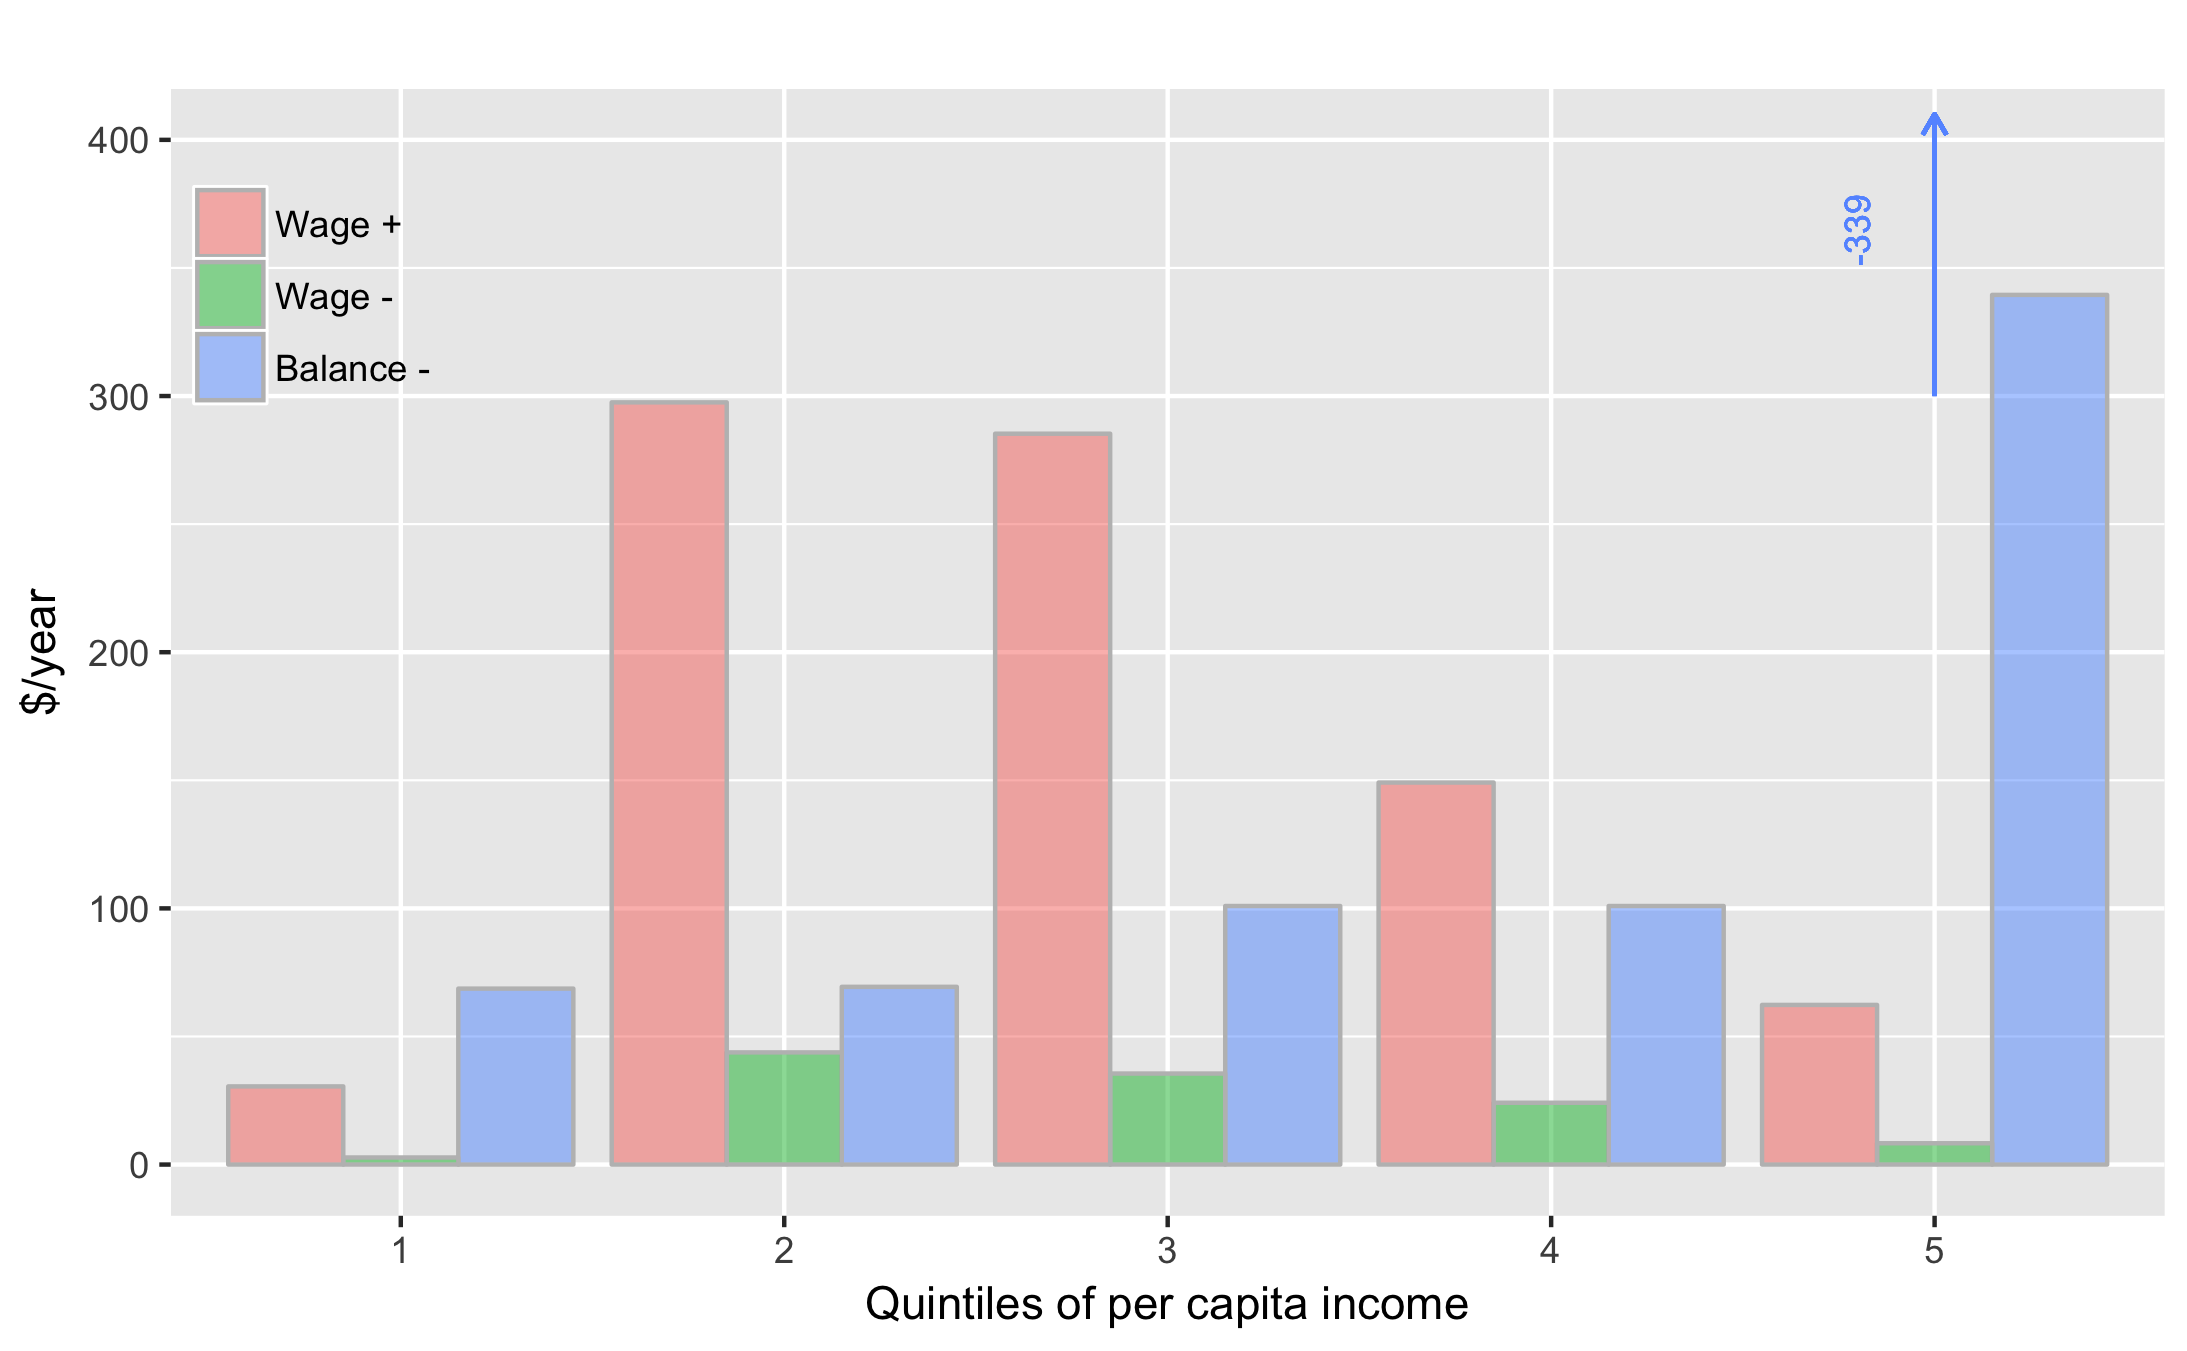
\includegraphics[scale = 0.13]{../Images/policy_est_bl_204040}
\caption{From $(1PL, 6PL) \sim (1\%, 29\%, 70\%)$ to  $(20\%, 40\%, 40\%)$}
\end{figure}	
\end{frame}

\begin{frame}{Comparing the Trade-offs: A Toy Example}

Model for the normative comparison made by a policy maker (welfare function):

\begin{align*}
W(\rho) &= \sum_{i \in N} \left( \omega_{wg}  wg_{i} + \omega_{wl} wl_{i} + \omega_{bl} bl_{i} \right) \omega^{d}_{i}(Q_{i}, \rho) \\
\text{with:}& \nonumber \\
\omega^{d}_{i}(Q_{i}, \rho) &= \frac{(1 - \rho(Q_{i} - Q_{median}) ) }{\sum_{i} \omega^{d}_{i}(Q_{i}) } Q_{max} \quad \text{for }  \rho \in \left(-\frac{1}{2}, \frac{1}{2} \right) \nonumber
\end{align*}
$\rho>0$ represent positive valuation of progressive redistribution. $\rho<0$ represents positive valuation of regressive redistribution (dis-utility from self loss greater than utility from others gain). 
\end{frame}


\begin{frame}{\hspace*{-2em} Normative Valuations and Redistribiutional Preferences  \linebreak \vspace*{-1em} Toy Example ({ $\omega_{WG} = \omega_{WL} = \omega_{BL} = 1$}) }

\vspace{-.2em}
\begin{figure}[h!]
\centering
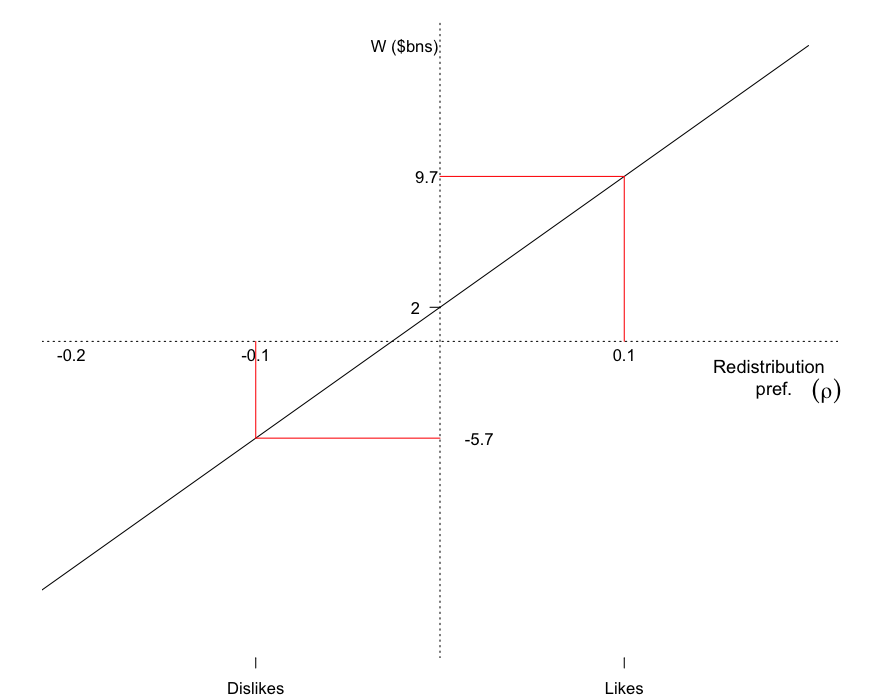
\includegraphics[scale = 0.35]{../Images/sample_pref}
\label{toy_ex}
\end{figure}	
\end{frame}



\begin{frame}{Sensitivity Analysis For Multiple Parameters}
\vspace*{-1.2em}
\begin{table}
\caption{$\%\Delta W$ for a $\%\Delta$ in inputs. Two sample policy makers: dislikes ($W(-0.1) = -\$5.3bn$) and likes ($W(0.1) = \$10.1bn$) redistribution}
\scalebox{0.7}{
\begin{tabular}{ll|c|c|c|c}
\hline
	   &						 & \multicolumn{4}{|c}{Re-distributional Preferences} \\
	   &						 & \multicolumn{2}{|c|}{Dislikes $(\rho = -0.1)$} & \multicolumn{2}{|c}{Likes $(\rho = 0.1)$} \\ \hline
Source & Input                & $10\% \Delta^{+}$ 	& $10\% \Delta^{-}$ & $10\% \Delta^{+}$ 	& $10\% \Delta^{-}$\\ \hline
\multicolumn{2}{l|}{Data}     &        &             		&  	\\
	& Annual wage growth ($g_{w}$)  	&	-3\% 	& 2\% 		&	-2\% 	& 1\%		\\
	& Annual growth in $N$ 			&	0.8\% 	& -0.9\%	 	&	0.5\% 	& -0.5\%	 \pause	\\
\multicolumn{2}{l|}{Research}        &        	&      	 	&	\\
    & $\eta_{teen}$     				&  -4\%    	&  4\%      &  -2\%    	&  2\%	    \pause \\
   	& Ripple Scope $(8.7, 11.5)$     &  37\%    	&  -24\%    &  21\%    &  -14\%	    \\
   	& Ripple Intensity $(50\% \Delta w)$& 5\%     &  -5\%     &  3\%     &  -3\%	   \pause \\
\multicolumn{2}{l|}{Guess Work}      &        	&          	&           \\
   	& Extrapolation factor ($F_{ex}$)&  -3\%    	&  2\%    	&  -1\%    &  1\%	    \\ 
   	& Non compliance ($\alpha_{1}$)  &  -7\%    	&  7\%      &  -4\%    &  4\%	    \\
   	& Substitution factor ($F_{sub}$)&      		&  20\%     &     		&  -8\%	    \\ 
   	& Net benefits					&    -5\%  	&  5\%      &     2\%  	&  -2\%	    \\
   	& Distribution of balance losses  &   \multicolumn{2}{c|}{}&    \multicolumn{2}{c}{} \\
    & Current: $(1\%, 29\%, 70\%)$	& 	\multicolumn{2}{c|}{} &   \multicolumn{2}{c}{} \pause\\
	& 	 $(1\%, 4\%, 95\%)$			&    \multicolumn{2}{c|}{22\%}     &    \multicolumn{2}{c}{13\%} 	    \\	 
  	& 	 $(5\%, 35\%, 60\%)$			&    \multicolumn{2}{c|}{-17\%}     &    \multicolumn{2}{c}{-9\%} 	    \\
  	& 	$1/N$						&    \multicolumn{2}{c|}{-129\%}     &    \multicolumn{2}{c}{-73\%}	   \\
\end{tabular}
}
\end{table}
\end{frame}


\begin{frame}{Welfare Effects: Elasticity of Labor Demand $W(\eta( F_{ext}, F_{adj},\eta_{lit}))$ }
\end{frame}

\begin{frame}[noframenumbering]{Welfare Effects: Elasticity of Labor Demand $W(\eta(\highlight{F_{ext}}, \highlightw{F_{adj}},\highlightw{\eta_{lit}}))$ }
\begin{figure}[h!]
\centering
\hspace{-1em}
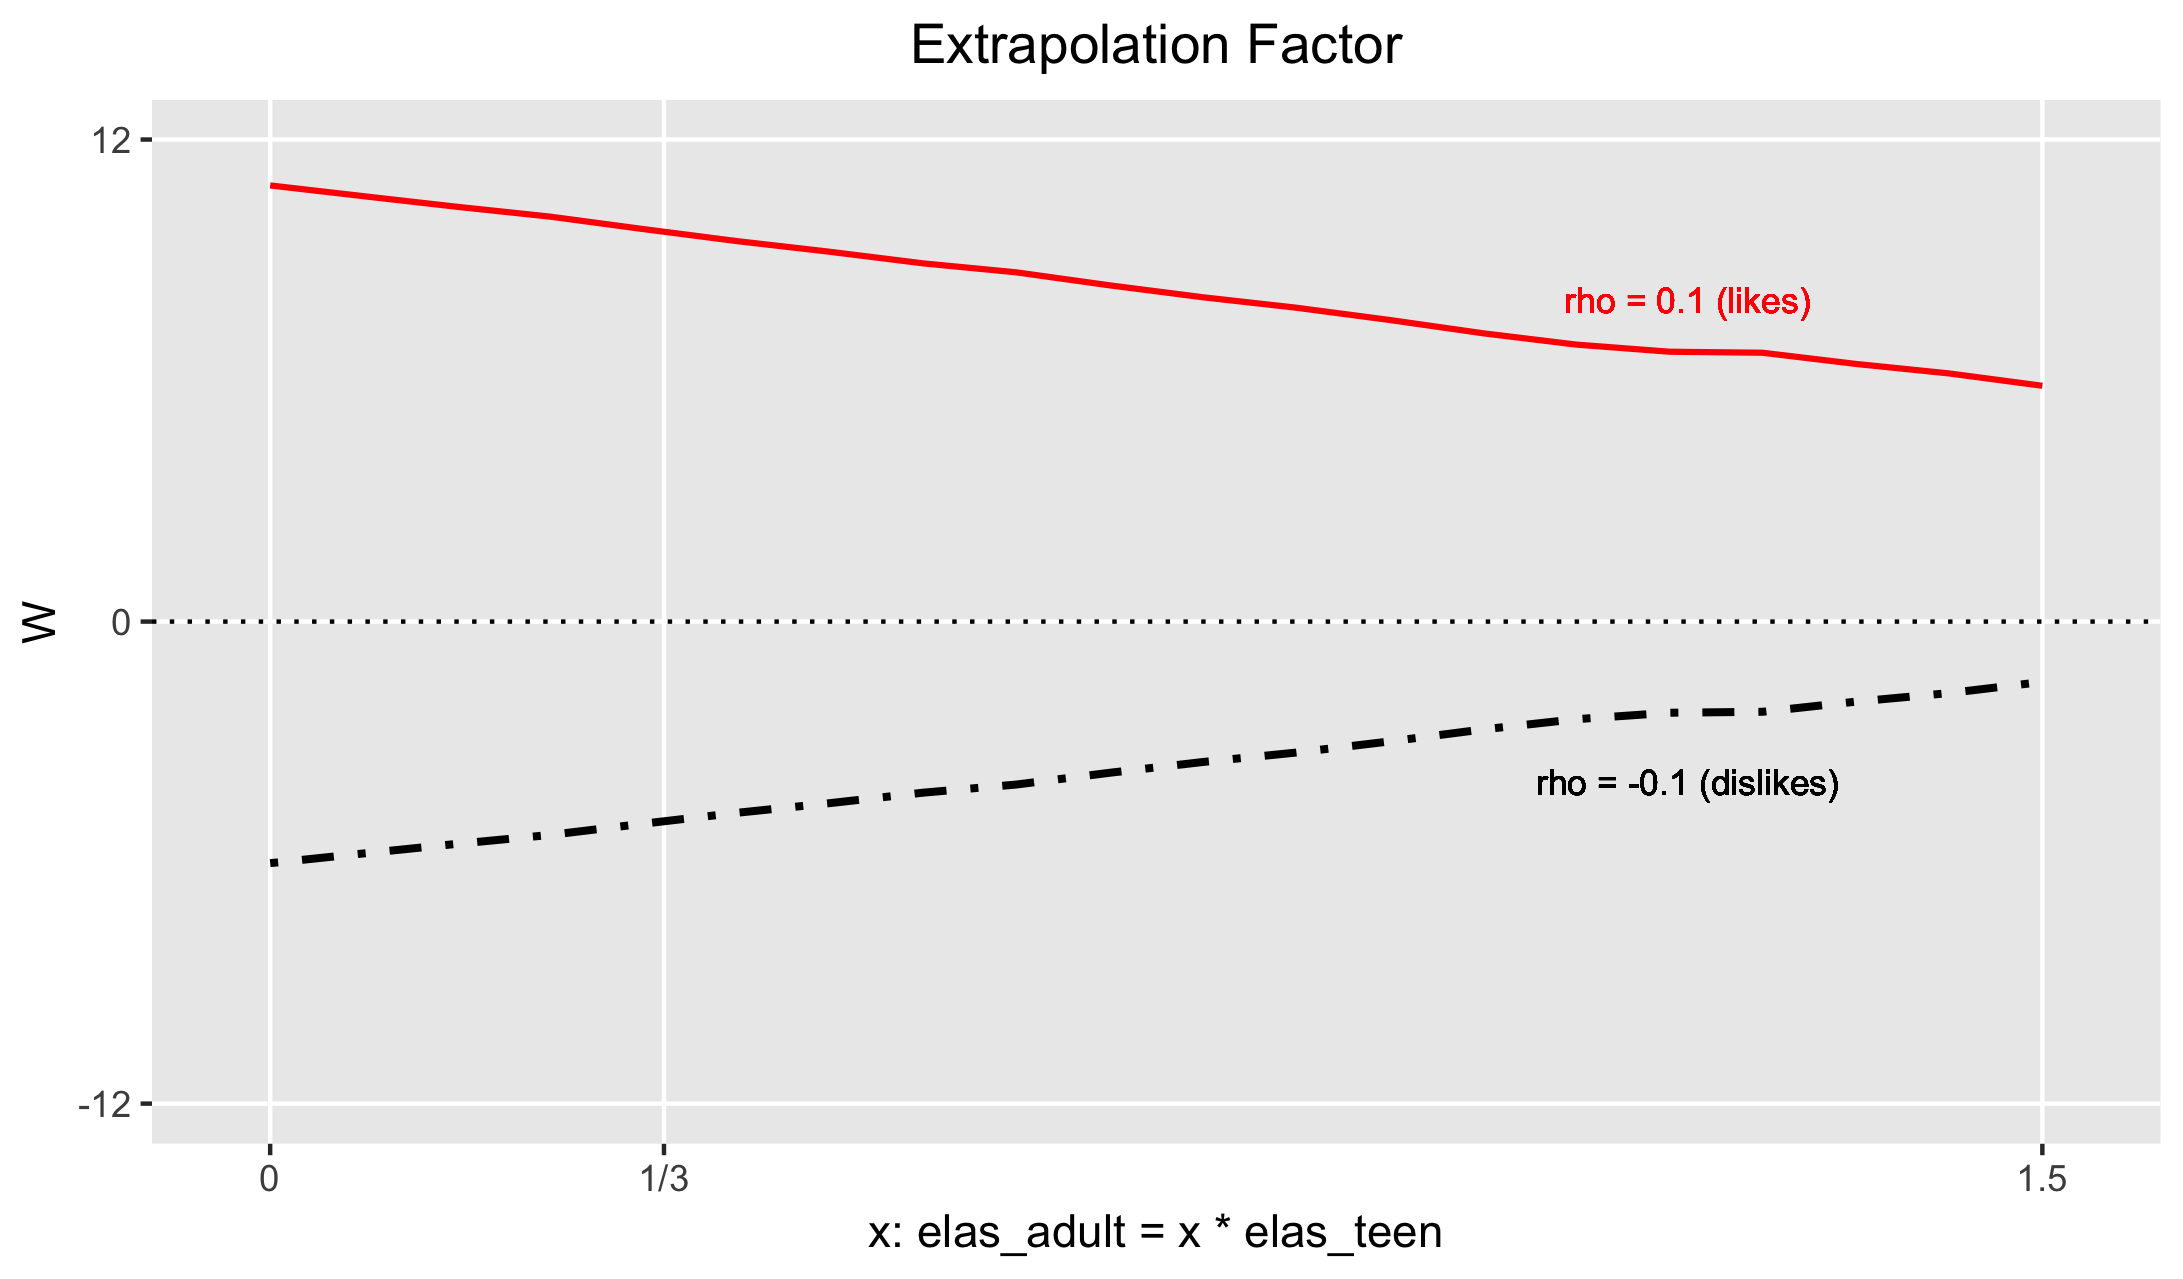
\includegraphics[scale = 0.13]{../Images/sa_extrap}
\end{figure}	
\end{frame}

\begin{frame}[noframenumbering]{Welfare Effects: Elasticity of Labor Demand $W(\eta( \highlightw{F_{ext}}, \highlight{F_{adj}},\highlightw{\eta_{lit}} ))$ }
\begin{figure}[h!]
\centering
\hspace{-1em}
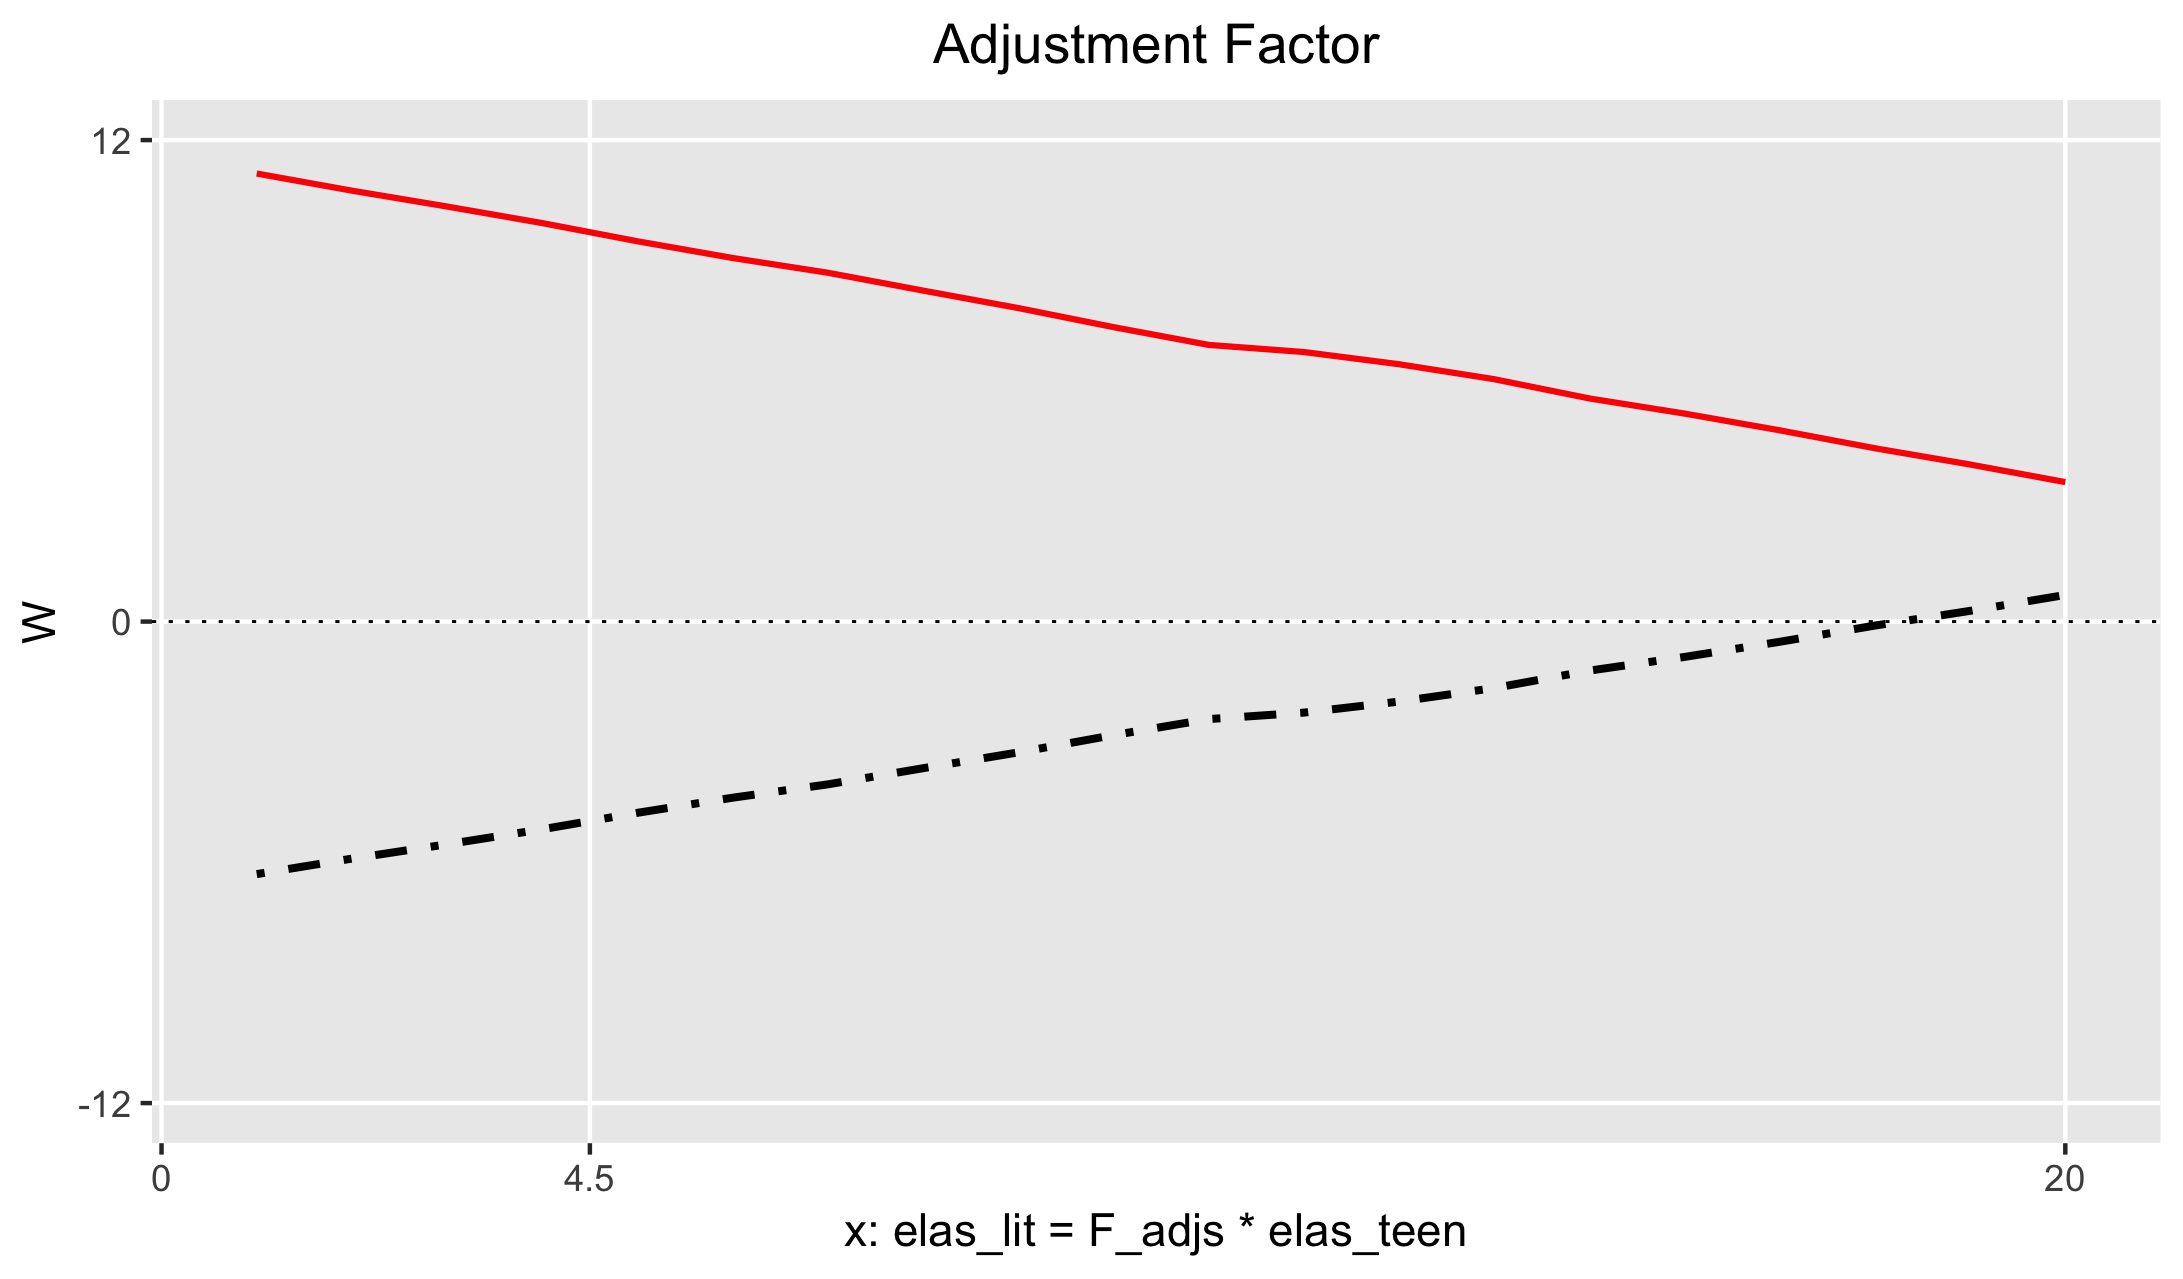
\includegraphics[scale = 0.13]{../Images/sa_f_adj}
\end{figure}	
\end{frame}

\begin{frame}[noframenumbering]{Welfare Effects: Elasticity of Labor Demand $W(\eta( \highlightw{F_{ext}}, \highlightw{F_{adj}},\highlight{\eta_{lit}}))$ }
\begin{figure}[h!]
\centering
\hspace{-1em}
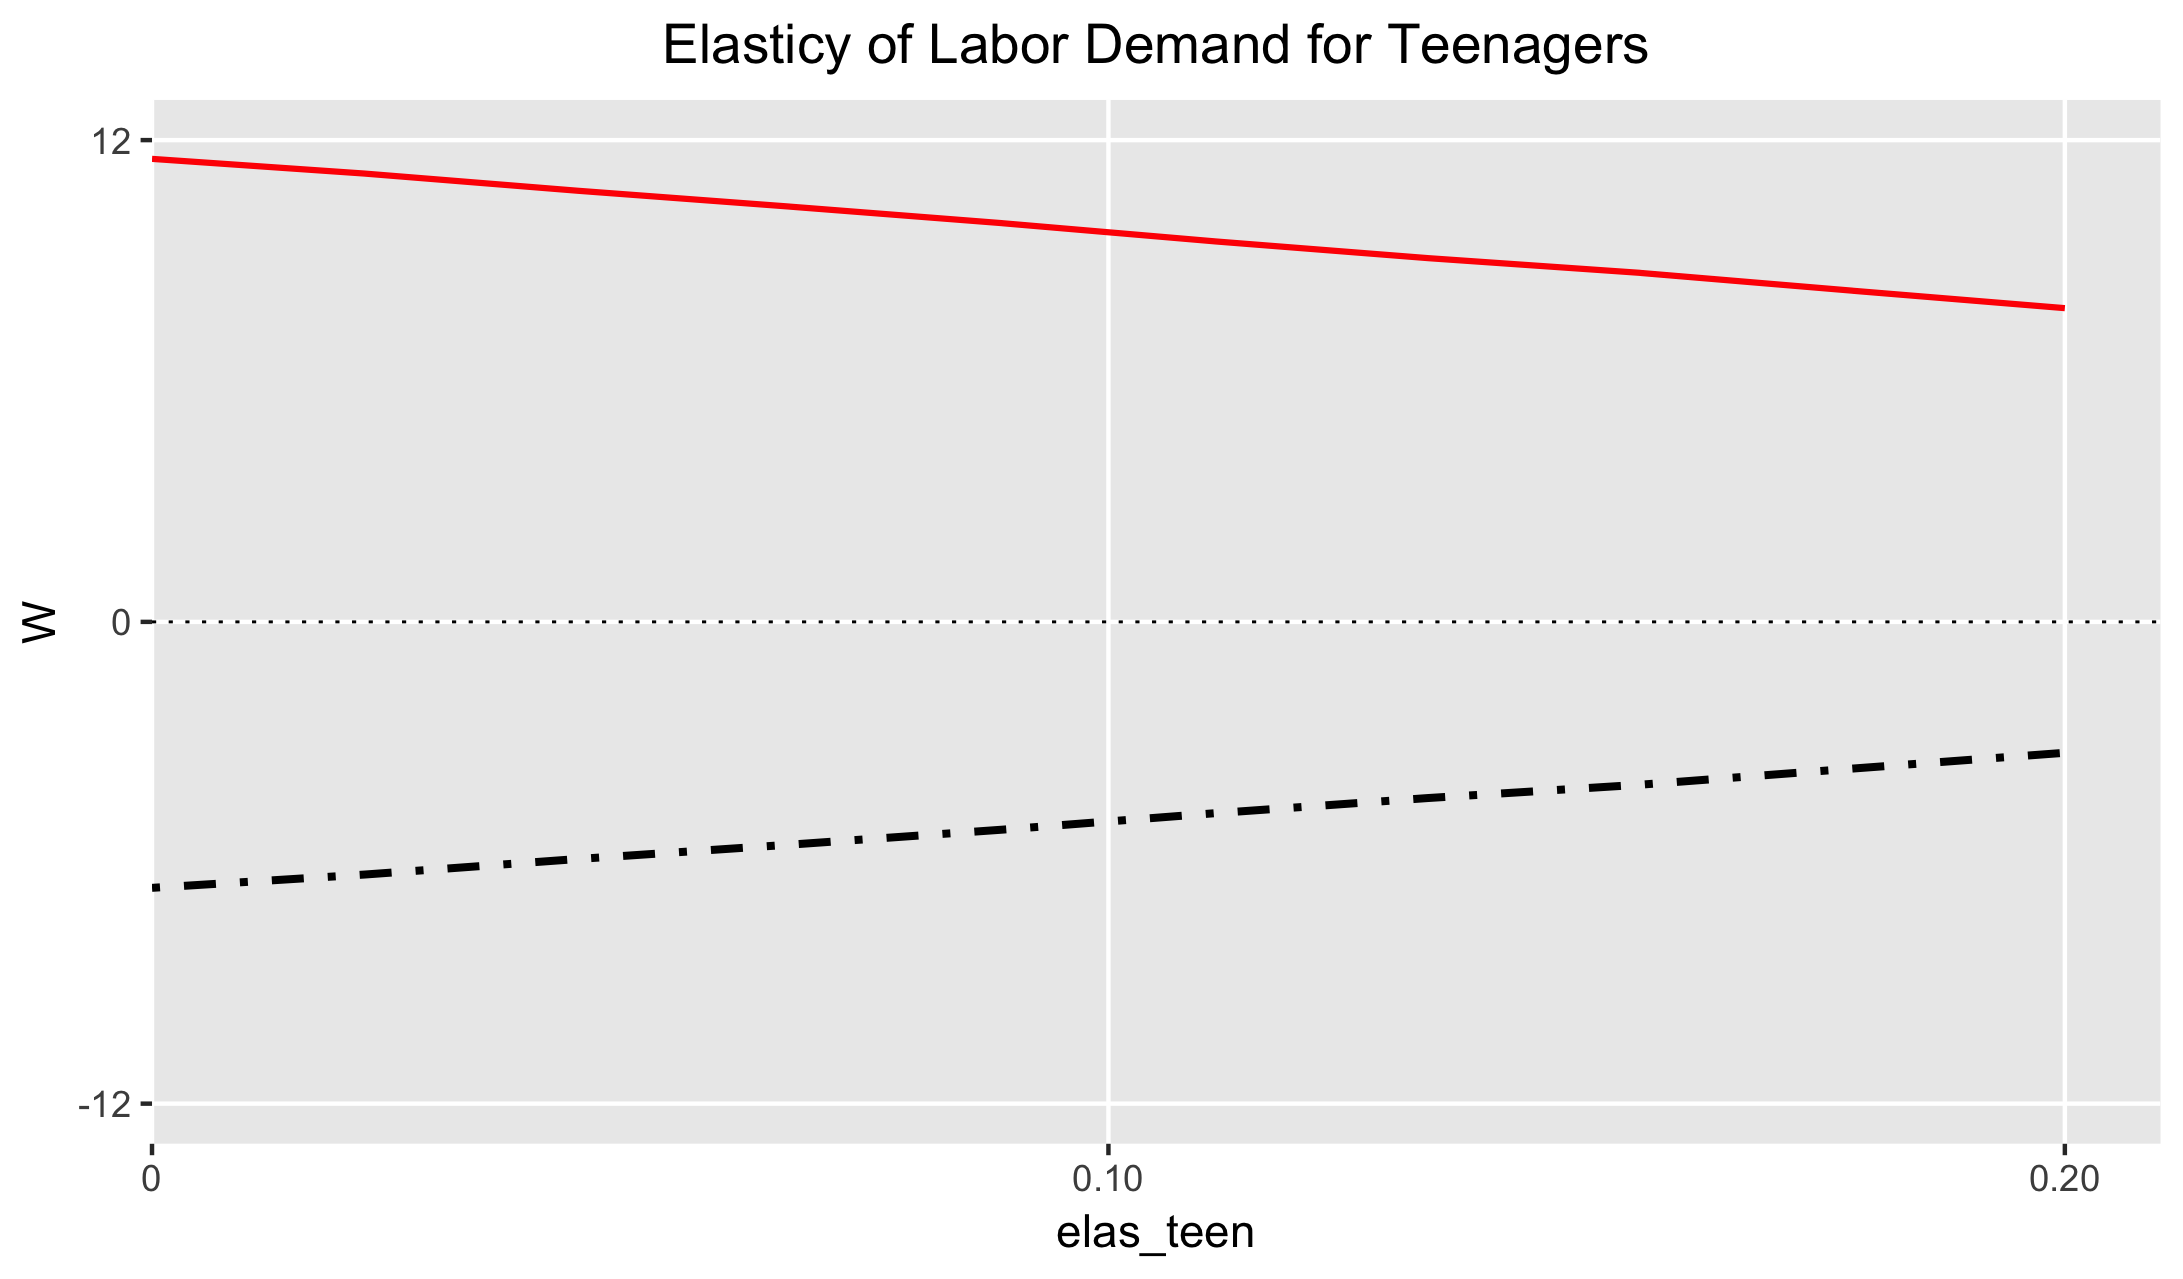
\includegraphics[scale = 0.13]{../Images/sa_eta}
\end{figure}	
\end{frame}



\begin{frame}{Much More Policy Relevant To Learn Who Pays For Wage Raise}
\begin{figure}[h!]
\vspace{-0em}
\centering
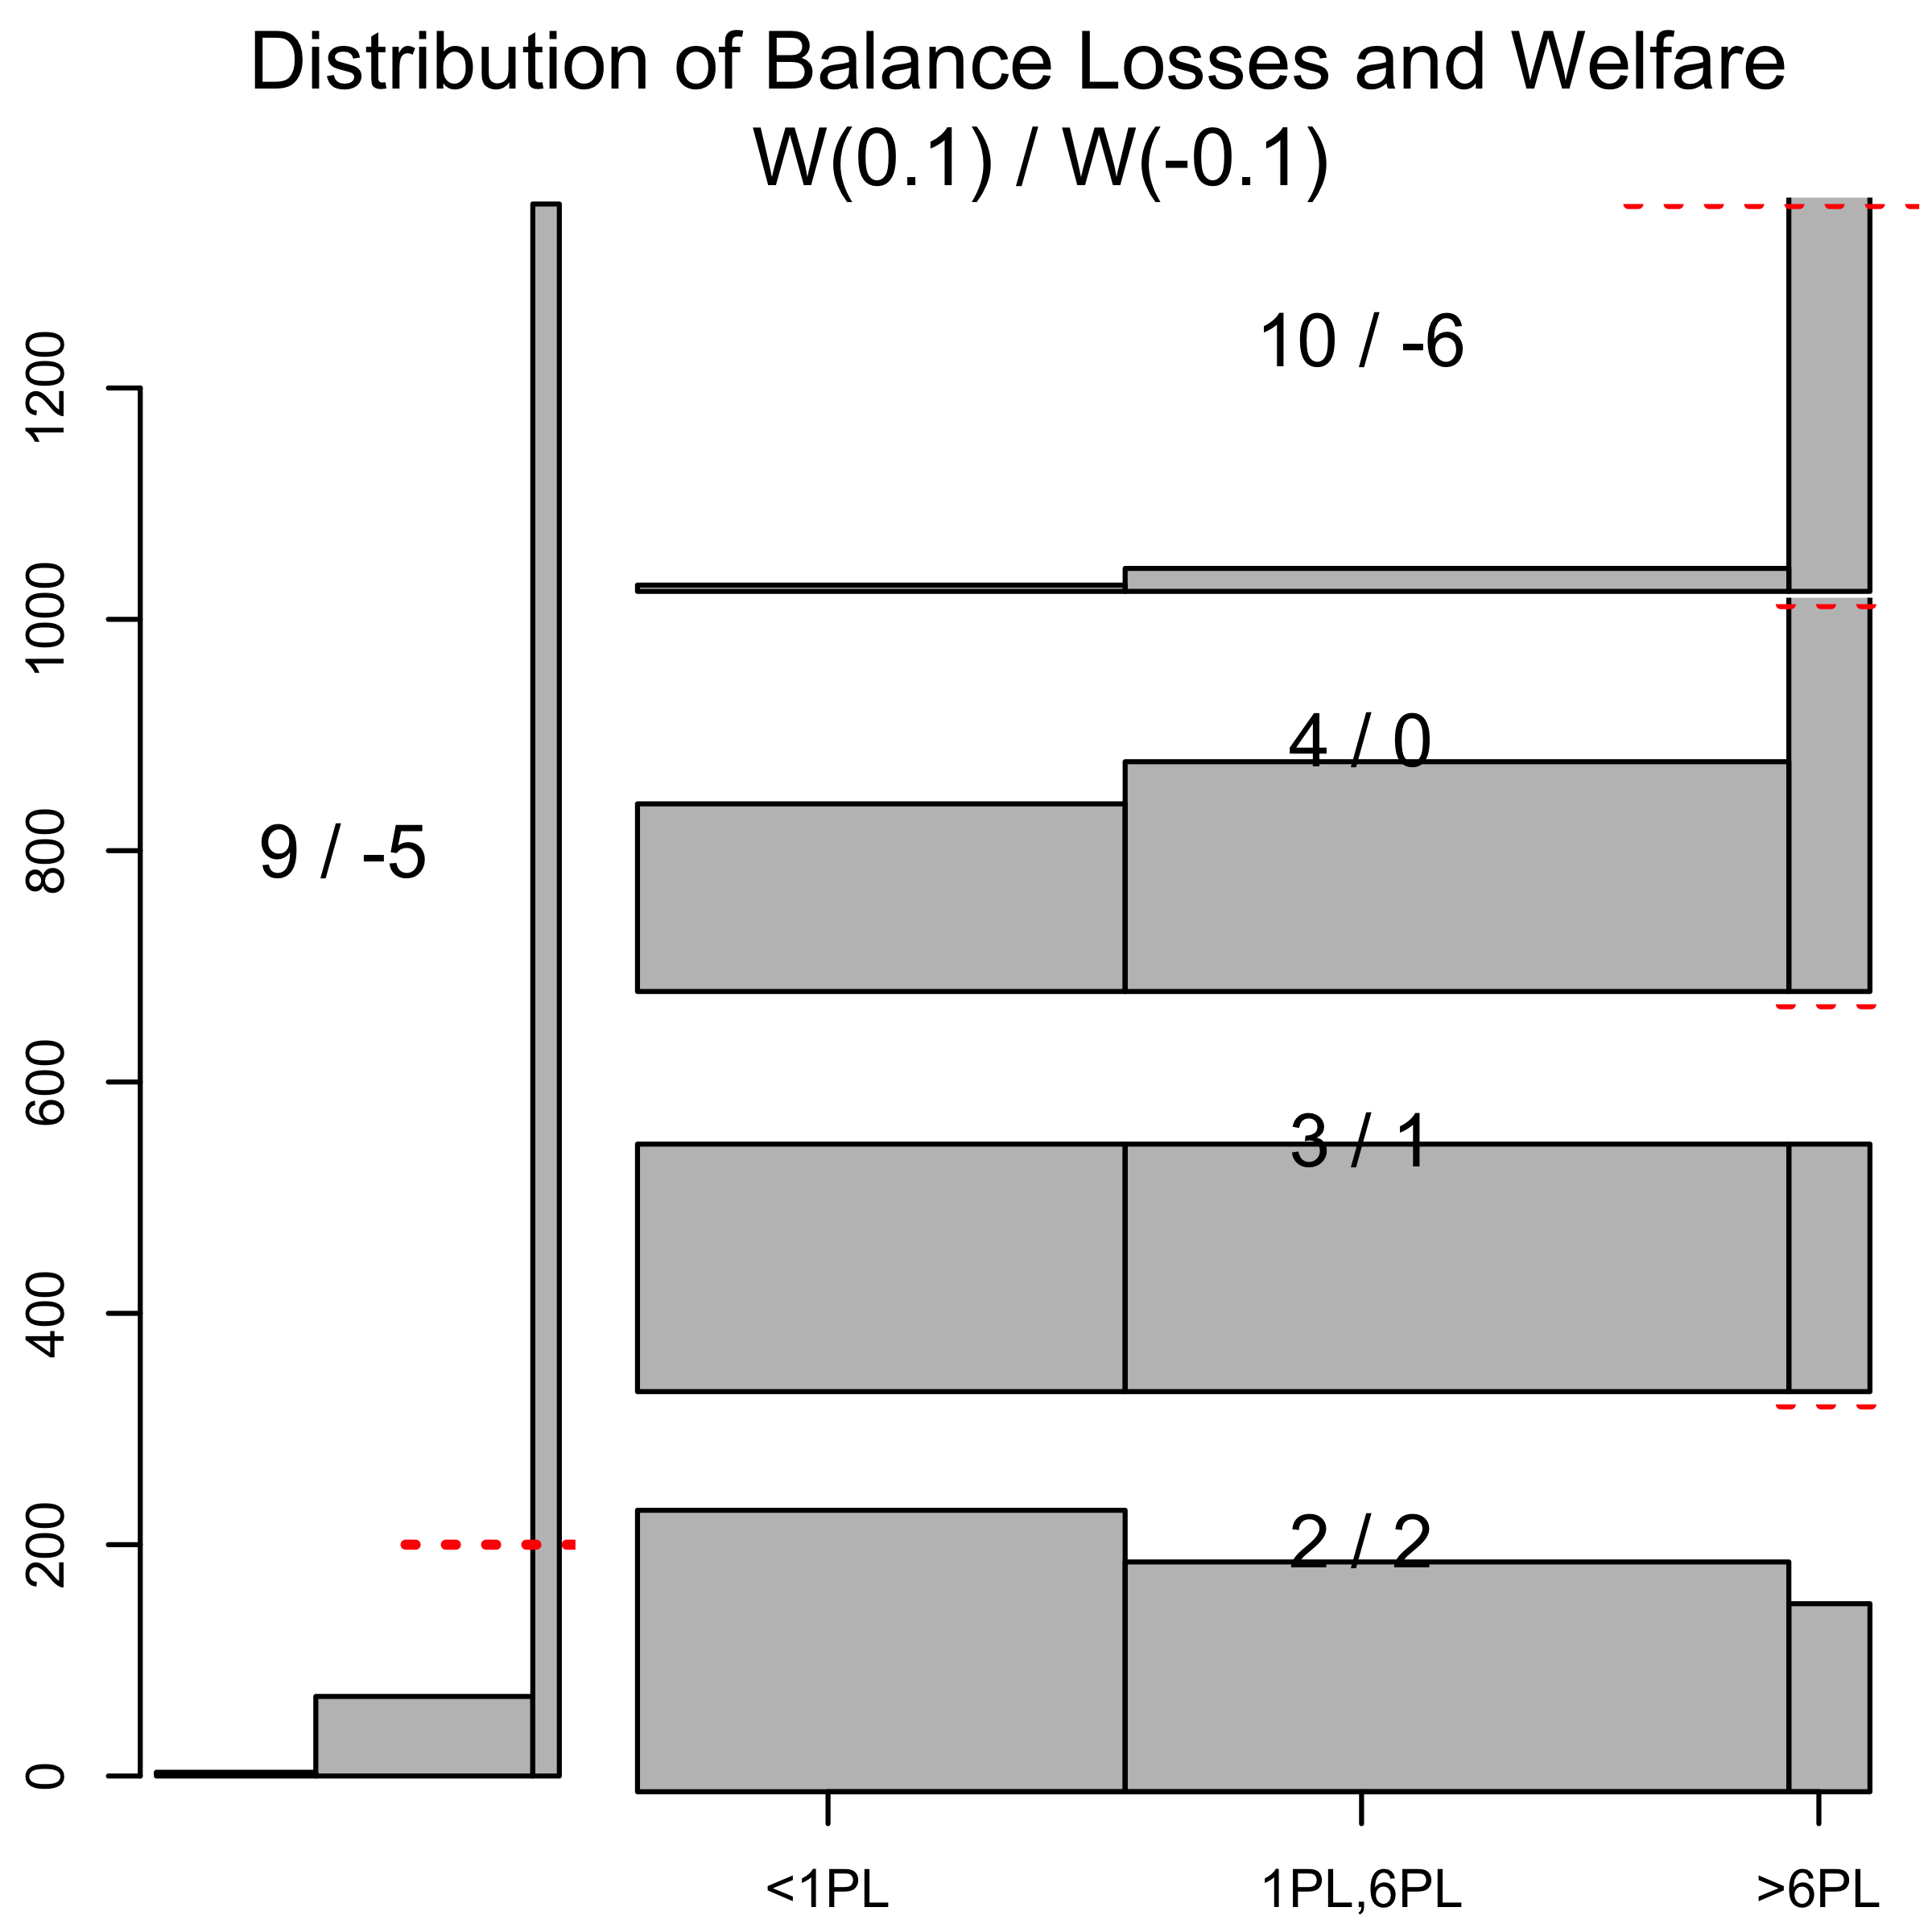
\includegraphics[scale = 0.09]{../Images/sa_DLf}
\label{SA_3}
\end{figure}	
\end{frame}

\section[Discussion]{Discussion and Next Steps}
% 5mins
\setbeamercovered{transparent}
\begin{frame}{Discussion}
\onslide<1>{
Let's assume this becomes the new status quo. 
\begin{itemize}
\item Costs of producing the next report on effects of min wage will be very small. 
\item Every additional effort will imply improvements on the ``state of the art'' report (e. g. $dBL$; $\eta(MW), \alpha_{1}(MW)$)
\item Learning about one parameter (QALYs, DWL) will update estimates \textit{across} reports.  
\item Much easier to have a substantive and normative policy debate (pilot example:\texttt{\href{https://fhoces.shinyapps.io/example_min_wage/}{Shiny App!}})

} 
%\onslide<2>{
%\item Two type of contributions ($\sim$software development):
%	\begin{itemize}
%	\item Short term: Within a given time period the model should be taken as given. Less freedom, but direct impact on the policy analysis. 
%	\item Long term: Structural revisions occur in parallel and are incorporated in future cycles of the analysis.
%	 	\end{itemize}
%}
%\onslide<2>{
%\item Who should work on this:
%\begin{itemize}
%\item Analytic reviewers of report; Research division within agencies; Study Commissions (``MWSC or MSWC?'' %\citep{card2016interview})
%\item Public policy schools. 
%\item Think tanks; Bank of knowledge \citep{clemens2016new}.
%\end{itemize}
%\item Next Steps
%\begin{itemize}
%\item BG: Reproduce meta-analysis and simulate new types of evidence; Improve DD; Incorporate %comments (especially from CBO); Deploy online (open source); Write!
%\item AG: $dBL$; $\eta(MW), \alpha_{1}(MW)$ and others ; \texttt{\href{https://%fhoces.shinyapps.io/example_min_wage/}{Shiny App!}}
%\end{itemize}

%}
\end{itemize}
\end{frame}

\begin{frame}{Next Steps}

\begin{itemize}
\item Publish a motivation/concept-note paper why and how do we need reproducible and transparent policy analysis
\item{\textbf{Find next case study, now with buy-in from a policy agency}}
\begin{itemize}
\item \textbf{Cost Benefit Analysis}
\item \textbf{Ex ante economic analysis/Micro-simulation study}
\end{itemize}
\item Review and publish guidelines
\end{itemize}
\end{frame}




\begin{frame}[shrink=30]{}



\tikzstyle{agent} = [diamond, draw, node distance= 7em, minimum height=5em, minimum width=5em]
\tikzstyle{line} = [draw, -stealth]

\tikzstyle{line_d} = [draw, dashed, -stealth]
\tikzstyle{inp} = [draw, circle, text centered, minimum height=2em, text width=2em, node distance= 10em]
\tikzstyle{outp} = [draw, circle, text centered, minimum height=2em, text width=2em, node distance= 10em]
\tikzstyle{block1} = [draw, circle,  text width=3em, text centered, minimum height=2em, node distance= 5em]
\tikzstyle{block2} = [draw, circle,  text width=4em, text centered, minimum height=2em, node distance= 5em]
\tikzstyle{block3} = [draw, rounded rectangle,  text width=5em, text centered, minimum height=2em, node distance= 5em]

\begin{figure}[h!]
\centering
\hspace*{0.2\linewidth}
\begin{tikzpicture}[thick,scale=0.2, every node/.style={scale=0.8}]

%% The oddly shaped truth
\node[regular polygon, regular polygon sides=3,
              draw, fill=white,
              inner sep=.1em,
              shape border rotate=70](tru){Truth};


%%%%%Researcher 1 and Inputs: depends on R_1%%%%%%%
\node [block1, right = 5em of tru](R_2){$R_2$};
\node [block1, above = 8em of R_2](R_1){$R_1$} node [left = -0.1em of R_1, text width = 5em]{Large Treatment Effect};
\node [block1, below = 8em of R_2](R_3){$R_3$} node [left = -0.1em of R_3, text width = 5em]{Small Treatment Effect};

\draw[decoration={brace,mirror}, decorate] (13,-33) -- node[below=6pt, text width = 4.8em](lab1){Researchers Degrees of 
Freedom}(18,-33);

\draw[decoration={brace,mirror}, decorate] (29,-33) -- node[below=6pt, text width = 4.8em](lab2){P. Analyst Degrees of 
Freedom}(34,-33);

\draw[decoration={brace}, decorate] (31,33) -- node[below=2pt]{Observed by citizens}(70,33);

%\node [agent](Researcher_1){$R_1$} node [left = 0.6em of Researcher_1, text width = 8em]{Large Treatment Effect};

\node [block1, right = 5em of R_1](PA_12){$PA_{1,2}$};
\node [block1, above = .5em of PA_12](PA_11){$PA_{1,1}$} node [right = -0.1em of PA_11, text width = 5em]{Large gains only};
\node [block1, below = .5em of PA_12](PA_13){$PA_{1,3}$};

\node [block1, right = 5em of R_2](PA_22){$PA_{22,}$};
\node [block1, above = .5em of PA_22](PA_21){$PA_{2,1}$};
\node [block1, below = .5em of PA_22](PA_23){$PA_{2,3}$};

\node [block1, right = 5em of R_3](PA_32){$PA_{3,2}$};
\node [block1, above = .5em of PA_32](PA_31){$PA_{3,1}$};
\node [block1, below = .5em of PA_32](PA_33){$PA_{3,3}$} node [right = -0.1em of PA_33, text width = 5em]{Large losses only};


\node [block2, above right = 3em and 15em of R_2](PM_1){Policy\linebreak Maker 1};
\node [block2, below right = 3em and 15em of R_2](PM_2){Policy\linebreak Maker 2};

\node [block3, right = 3em of PM_1](PC_1){Support};
\node [block3, right = 3em of PM_2](PC_2){Oppose};


%%%%% Draw edges col 2%%%%%%%%%%%%%%%%%
%Truth to research
\draw [line](tru) -- (R_1);
\draw [line_d](tru) -- (R_2);
\draw [line_d](tru) -- (R_3);


%Research  to PA
\draw [line_d](R_1) -- (PA_13);
\draw [line_d](R_1) -- (PA_11);
\draw [line](R_1) -- (PA_12);

\draw [line_d](R_2) -- (PA_23);
\draw [line_d](R_2) -- (PA_21);
\draw [line_d](R_2) -- (PA_22);

\draw [line_d](R_3) -- (PA_33);
\draw [line_d](R_3) -- (PA_31);
\draw [line_d](R_3) -- (PA_32);



%PA to PM
\draw [line](PA_11) -- (PM_1);
\draw [line](PA_33) -- (PM_2);
%PM to PC
\draw [line](PM_1) -- (PC_1);
\draw [line](PM_2) -- (PC_2);

\node[draw=red,rounded corners = 1ex,fit=(PA_11)(PA_33),inner sep = 44pt](redb){};
\node [right = 5em of PA_22,color=red, text width = 8em](t_redb){\Huge Are you here?};
\draw [line, color=red](redb) -- (t_redb);

%%%%%%%%%%%%%%%%%%%%%%%%%%%%%%%%%%%%%%




\end{tikzpicture}
\caption{Policy-making with low TR in research and policy analysis}\label{low_cred}
\end{figure}
%\end{comment}
\end{frame}



\begin{frame}[shrink=30, noframenumbering]{}



\tikzstyle{agent} = [diamond, draw, node distance= 7em, minimum height=5em, minimum width=5em]
\tikzstyle{line} = [draw, -stealth]

\tikzstyle{line_d} = [draw, dashed, -stealth]
\tikzstyle{inp} = [draw, circle, text centered, minimum height=2em, text width=2em, node distance= 10em]
\tikzstyle{outp} = [draw, circle, text centered, minimum height=2em, text width=2em, node distance= 10em]
\tikzstyle{block1} = [draw, circle,  text width=3em, text centered, minimum height=2em, node distance= 5em]
\tikzstyle{block2} = [draw, circle,  text width=4em, text centered, minimum height=2em, node distance= 5em]
\tikzstyle{block3} = [draw, rounded rectangle,  text width=5em, text centered, minimum height=2em, node distance= 5em]

\begin{figure}[h!]
\centering
\hspace*{0.2\linewidth}
\begin{tikzpicture}[thick,scale=0.2, every node/.style={scale=0.8}]

%% The oddly shaped truth
\node[regular polygon, regular polygon sides=3,
              draw, fill=white,
              inner sep=.1em,
              shape border rotate=70](tru){Truth};


%%%%%Researcher 1 and Inputs: depends on R_1%%%%%%%
\node [block1, right = 5em of tru](R_2){$R_2$};
\node [block1, above = 8em of R_2](R_1){$R_1$} node [left = -0.1em of R_1, text width = 5em]{Large Treatment Effect};
\node [block1, below = 8em of R_2](R_3){$R_3$} node [left = -0.1em of R_3, text width = 5em]{Small Treatment Effect};

\draw[decoration={brace,mirror}, decorate] (13,-33) -- node[below=6pt, text width = 4.8em](lab1){Researchers Degrees of 
Freedom}(18,-33);

\draw[decoration={brace,mirror}, decorate] (29,-33) -- node[below=6pt, text width = 4.8em](lab2){P. Analyst Degrees of 
Freedom}(34,-33);

\draw[decoration={brace}, decorate] (31,33) -- node[below=2pt]{Observed by citizens}(70,33);

%\node [agent](Researcher_1){$R_1$} node [left = 0.6em of Researcher_1, text width = 8em]{Large Treatment Effect};

\node [block1, right = 5em of R_1](PA_12){$PA_{1,2}$};
\node [block1, above = .5em of PA_12](PA_11){$PA_{1,1}$} node [right = -0.1em of PA_11, text width = 5em]{Large gains only};
\node [block1, below = .5em of PA_12](PA_13){$PA_{1,3}$};

\node [block1, right = 5em of R_2](PA_22){$PA_{22,}$};
\node [block1, above = .5em of PA_22](PA_21){$PA_{2,1}$};
\node [block1, below = .5em of PA_22](PA_23){$PA_{2,3}$};

\node [block1, right = 5em of R_3](PA_32){$PA_{3,2}$};
\node [block1, above = .5em of PA_32](PA_31){$PA_{3,1}$};
\node [block1, below = .5em of PA_32](PA_33){$PA_{3,3}$} node [right = -0.1em of PA_33, text width = 5em]{Large losses only};


\node [block2, above right = 3em and 15em of R_2](PM_1){Policy\linebreak Maker 1};
\node [block2, below right = 3em and 15em of R_2](PM_2){Policy\linebreak Maker 2};

\node [block3, right = 3em of PM_1](PC_1){Support};
\node [block3, right = 3em of PM_2](PC_2){Oppose};


%%%%% Draw edges col 2%%%%%%%%%%%%%%%%%
%Truth to research
\draw [line](tru) -- (R_1);
\draw [line_d](tru) -- (R_2);
\draw [line_d](tru) -- (R_3);


%Research  to PA
\draw [line_d](R_1) -- (PA_13);
\draw [line_d](R_1) -- (PA_11);
\draw [line](R_1) -- (PA_12);

\draw [line_d](R_2) -- (PA_23);
\draw [line_d](R_2) -- (PA_21);
\draw [line_d](R_2) -- (PA_22);

\draw [line_d](R_3) -- (PA_33);
\draw [line_d](R_3) -- (PA_31);
\draw [line_d](R_3) -- (PA_32);



%PA to PM
\draw [line](PA_11) -- (PM_1);
\draw [line](PA_33) -- (PM_2);
%PM to PC
\draw [line](PM_1) -- (PC_1);
\draw [line](PM_2) -- (PC_2);

\node[draw=red,rounded corners = 1ex,fit=(PA_12),inner sep = 14pt](redb){};
\node [right = 5em of PA_12,color=red, text width = 16em](t_redb){ \Huge Would you like to show that you are here?};
\draw [line, color=red](redb) -- (t_redb);

%%%%%%%%%%%%%%%%%%%%%%%%%%%%%%%%%%%%%%




\end{tikzpicture}
\caption{Policy-making with low TR in research and policy analysis}\label{low_cred}
\end{figure}
%\end{comment}
\end{frame}

\begin{frame}[noframenumbering]
\begin{center}
\vspace*{4em}
{\Large Thank you.\\}
\bigskip
Pre-print: [PP URL HERE]   \\
Contact:  \href{mailto:fhoces@berkeley.edu}{fhoces@berkeley.edu}

\end{center}
\end{frame}

\appendix

\begin{frame}[noframenumbering]
\begin{center}
Back-up slides
\end{center}
\end{frame}








\backupbegin


\bibliography{../resources/motivation_paper}
\bibliographystyle{plainnat}





\begin{frame}[label=equations]{{\small\hyperlink{map_cbo}{\beamerbutton{}}}Equations from Model in DD}
\subsection{Employment}

\begin{flalign}\label{N_final}
\widehat{\Delta E} &= N \times \eta \times \% \Delta w  + \text{Other factors} &&
\end{flalign}

\begin{flalign}
\widehat{ N^{s}_{final} } &= \hat{ g_{N}(t'|t) } \times  \hat{ N^{s}_{t} }  \times P(\hat{w'} \leq MW^{new}|s)  \times (1 - \hat{ \alpha^{s}_{1} } - \hat{ \alpha^{s}_{2} })  \hspace{2em} s = \{teens, \, adults \} &&
\end{flalign}

The elasticity for adults from the literature is define as the one for teenagers with an extrapolation factor. 
  
\begin{flalign}
\eta^{adults}_{lit} &= \eta^{teens}_{lit} \times F_{extrapolation}&& 
\end{flalign}
\end{frame}

\begin{frame}{{\small\hyperlink{map_cbo}{\beamerbutton{}}}Adjustments to the elasticity of labor demand}
Following \cite{neumark2008minimum, brown1999minimum}. First:

\begin{flalign}
\eta^{s}_{lit} &= p^{s}_{w\leq MW} \eta^{s}_{w\leq MW} + (1 - p^{s}_{w\leq MW})\eta^{s}_{w > MW}  \hspace{2em} s = \{teens, \, adults \} &&\nonumber 
\end{flalign}

Second, assume $\eta^{s}_{w\leq MW} = 0$:

\begin{flalign}
\eta^{s}_{w\leq MW} &= \frac{\eta^{s}_{lit}}{p^{s}_{w\leq MW}}  \hspace{2em} s = \{teens, \, adults \}&& \nonumber
\end{flalign}

And third, adjust for the effective average wage variation for each group ($\overline{\%\Delta w^{s}}$):

\begin{flalign}\label{eta_final}
\widetilde{ \eta^{s}_{w\leq MW} } &=  \frac{\eta^{s}_{lit}}{p^{s}_{w\leq MW}} \times \frac{\%\Delta MW}{\overline{\%\Delta w^{s}}} = \eta^{s}_{lit} \times F^{s}_{adjs}  \hspace{2em} s = \{teens, \, adults \}&&
\end{flalign}

\end{frame}


\begin{frame}{{\small\hyperlink{map_cbo}{\beamerbutton{}}}Final Effect on Employment}

\begin{flalign}
 \widehat{ \Delta E } &= \sum_{g\in\{A,T\}} \left( \widehat{ N^{final}_{g} } \times \widetilde{ \eta^{g}_{w\leq MW} }\times \overline{\%\Delta w^{g}}  \right) - \widehat{OF}&&
\end{flalign}
\end{frame}

\begin{frame}{{\small\hyperlink{map_cbo}{\beamerbutton{}}}Effect on Wages}
\subsection{Wages}  

\begin{flalign}\label{no_comp}
w^{''} &=
\begin{cases}
w' \quad if \quad  w \in U[0,1]<\alpha_1 \\
w^{new} \quad \quad o/w
\end{cases} &&
\end{flalign}

\begin{flalign}
w^{new} &=
\begin{cases}
w'/2 \quad if \quad  w \in U[0,1]<\alpha_{aux} \\
\widetilde{w^{new}} \quad \quad o/w
\end{cases} &&
\end{flalign}

Ripple Effects

\begin{flalign}\label{ripple_wages}
\widetilde{w^{new}}  &=
\begin{cases}
MW' \quad if \quad  w' < R_{lb} \\
MW' + R^{I}(w' - R^{s}_{lb} )\quad if \quad  w' \in [R_{lb}, MW') \\
w' + R^{I}(R^{s}_{ub} - w' )\quad if \quad  w' \in [MW', R_{ub}) \\
w' \quad \quad o/w
\end{cases} &&
\end{flalign}
\end{frame}

\begin{frame}{{\small\hyperlink{map_cbo}{\beamerbutton{}}}Computing Income}
\vspace{-0.5em}
\subsection{Income}

\begin{flalign}
 y'_{i,h} &= \sum_{i\in N_{h}} \left( g_{nw}(t'|t) nw_{i} + w'_{i}  \right)/N_{h} &&\nonumber \\
 y''_{i,h} &= \sum_{i\in N_{h}} \left( g_{nw}(t'|t) nw_{i} + w''_{i}  \right)/N_{h} &&
\end{flalign}

\textbf{Final Policy Estimates}
\vspace{-0.5em}
\begin{flalign}
 WG_{i} &=  \left(y''_{i}  - y'_{i} \right) \mathbf{I}\left(y''_{i}  > y'_{i} \right)  &&\\
 WL_{i} &=  \left(y'_{i}  - y"'_{i} \right) \mathbf{I}\left(y''_{i}  < y'_{i} \right)  && \\
 BL &= \sum_{i} WG_{i} - F_{sub} \sum_{i} WL_{i};\quad 
 BL_i = BL \times dBL &&\\
 \overline{WG_{Q}} &= \frac{\sum_{i \in Q} WG_{i}}{N_{pop}/5} \quad
 \overline{WL_{Q}} = \frac{\sum_{i \in Q} WL_{i}}{N_{pop}/5}  && \nonumber\\ 
 \overline{BL_{Q}} &= \frac{\sum_{i \in Q} BL_{i}}{N_{pop}/5} &&\label{last.eq}  
\end{flalign}

\end{frame}


\begin{frame}[plain, label=no_inet]{Snapshots of DD}
\vspace{-2em}
\begin{figure}[h!]
\centering
\hspace{-5em} 
\includegraphics[scale = 0.28]{../Images/Screen_Shot1}
\hyperlink{demo}{\beamerbutton{}}
\end{figure}	

\end{frame}

\begin{frame}[plain]{Snapshots of DD\hyperlink{demo}{\beamerbutton{}}}
\vspace{-2em}
\begin{figure}[h!]
\centering
\hspace{-5em} 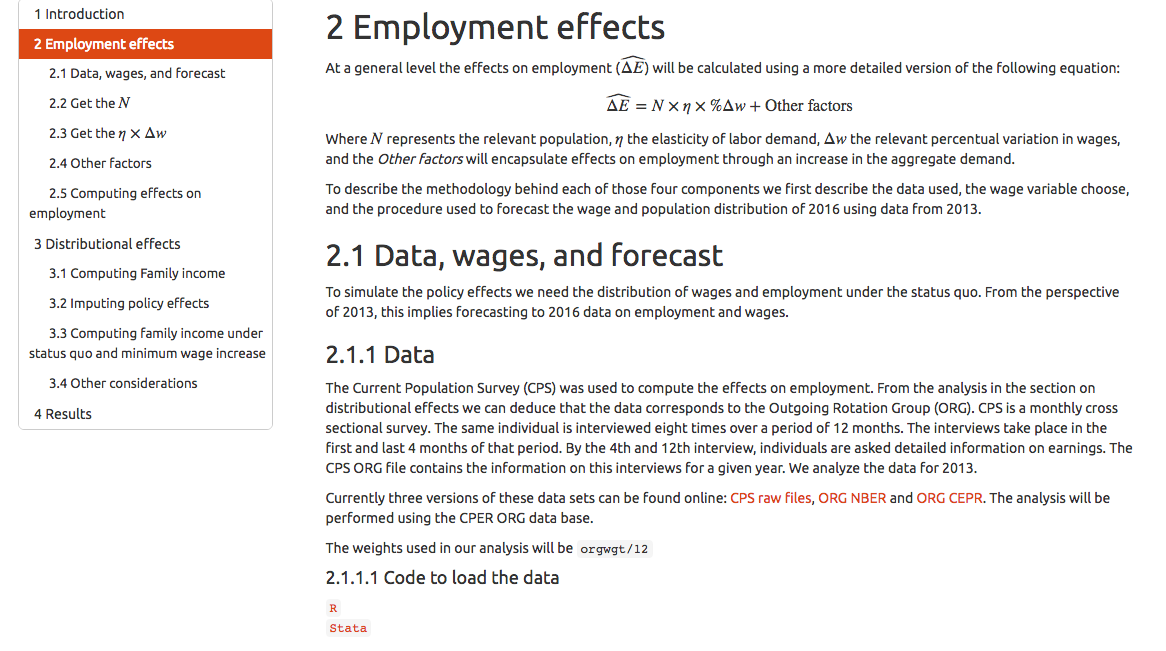
\includegraphics[scale = 0.28]{../Images/Screen_Shot2}
\hyperlink{demo}{\beamerbutton{}}
\end{figure}	
\end{frame}

\begin{frame}[plain]{Snapshots of DD\hyperlink{demo}{\beamerbutton{}}}
\vspace{-2em}
\begin{figure}[h!]
\centering
\hspace{-5em} 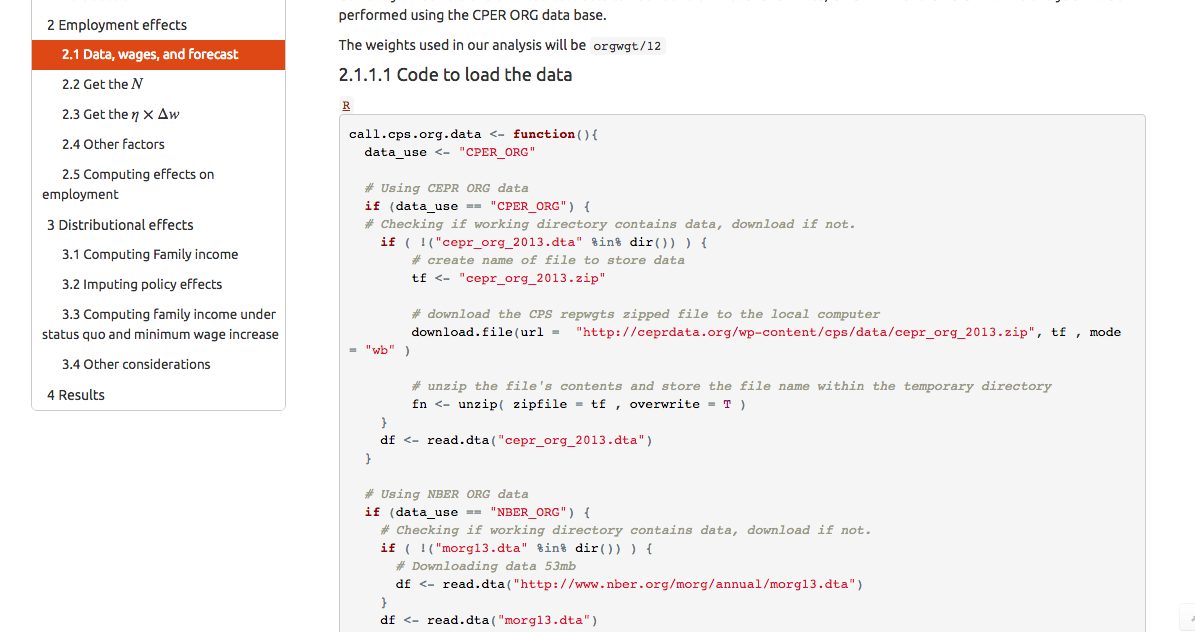
\includegraphics[scale = 0.28]{../Images/Screen_Shot3}
\hyperlink{demo}{\beamerbutton{}}
\end{figure}	
\end{frame}

\begin{frame}[plain]{Snapshots of DD\hyperlink{demo}{\beamerbutton{}}}
\vspace{-2em}
\begin{figure}[h!]
\centering
\hspace{-5em} 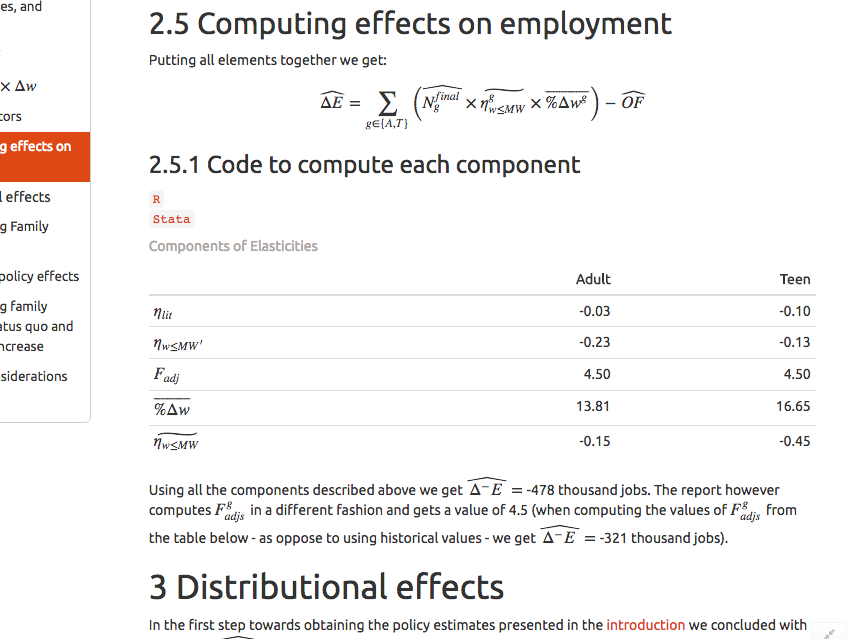
\includegraphics[scale = 0.28]{../Images/Screen_Shot4}
\hyperlink{demo}{\beamerbutton{}}
\end{figure}	
\end{frame}

\begin{frame}[plain]{Snapshots of DD\hyperlink{demo}{\beamerbutton{}}}
\vspace{-2em}
\begin{figure}[h!]
\centering
\hspace{-5em} 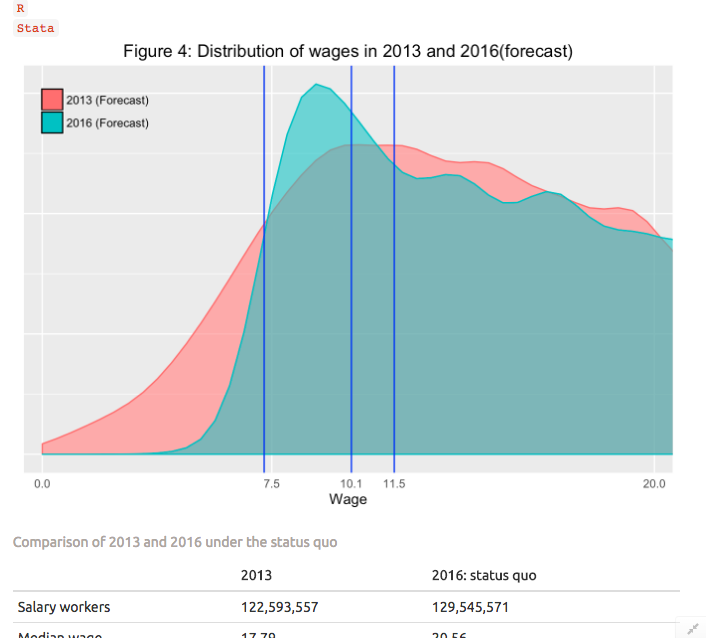
\includegraphics[scale = 0.28]{../Images/Screen_Shot5}
\hyperlink{demo}{\beamerbutton{}}
\end{figure}	
\end{frame}

\begin{frame}[plain]{Snapshots of DD}
\vspace{-2em}
\begin{figure}[h!]
\centering
\hspace{-5em} 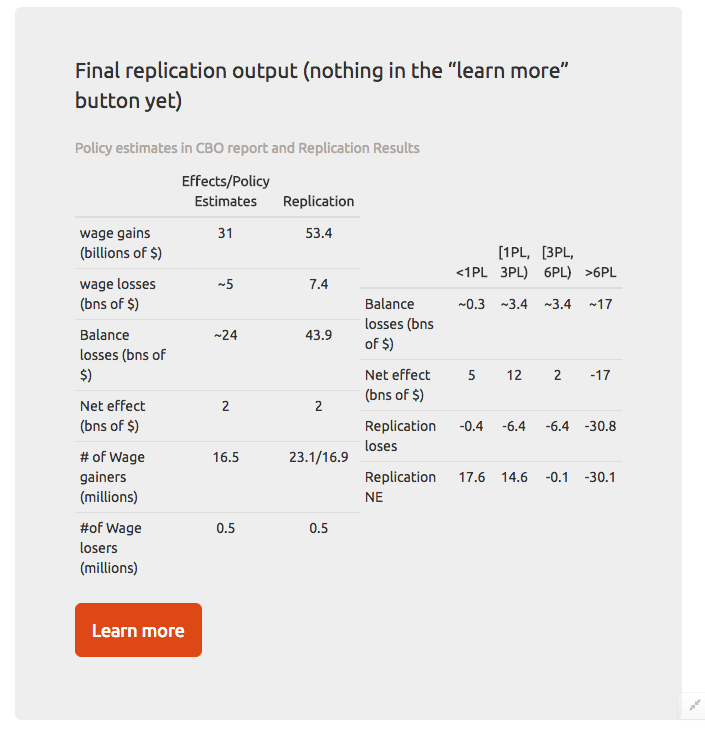
\includegraphics[scale = 0.28]{../Images/Screen_Shot6}
\hyperlink{demo}{\beamerbutton{}}
\end{figure}	
\end{frame}


\backupend


 \end{document}